%!TEX root = Masterarbeit.tex
% Hier k�nnen die einzelnen Kapitel inkludiert werden. Sie m�ssen in den 
% entsprechenden .TEX-Dateien vorliegen. Die Dateinamen k�nnen nat�rlich 
% angepasst werden.

%!TEX root = ../Masterarbeit.tex
\chapter{Einleitung}
\label{cha:Einleitung}

\section{Motivation}
Die Idee f�r diese Arbeit ist beim H�ren eines �lteren Musiktitels entstanden. Hierbei entstand der Wunsch danach zu diesem Zeitpunkt einen Radiosender h�ren zu k�nnen, wie er sich zu der Zeit der Popularit�t des Musiktitels angeh�rt h�tte. Dabei m�sste in Betracht gezogen werden, welche Lieder bereits zu diesem Zeitpunkt popul�r gewesen sind, bzw. welche zuk�nftigen Hits vielleicht schon im Radio gespielt worden sind. Dies allein l�sst sich mehr oder weniger simpel mit alten Musiksamplern \ua abdecken. Interessant wird es jedoch dann, wenn der Zeitpunkt als eine Art Epoche betrachtet und dargestellt wird. \Dahe dass �ber passende Musiktitel hinaus weitere Medientypen mit relevanten Inhalten in die Darstellung aufgenommen werden, um sich ein m�glichst umfassendes Bild des Zeitgeschehens zum gew�hlten Zeitpunktes machen zu k�nnen, welches  sowohl informativ, als auch emotional anspricht. \todo{emotional. really?}

\section{Ziel und Abgrenzung dieser Arbeit}
Die Herausforderung dieser Arbeit ist es, eine Web-Anwendung zu implementieren, die es dem Nutzer erlaubt anhand eines Datums, Informationen verschiedener Medientypen aus dieser Zeit anzeigen zu lassen. Diese Informationen sollen sowohl Musik, als auch Bilder, Videos und Neuigkeiten beinhalten. Hierbei sollen zeitlich voneinander abh�ngige und thematisch verwandte Daten dargestellt werden. So kann \zB ein zu der Zeit aufgetretenes wichtiges Ereignis in Form eines Wikipedia-Artikels dargestellt werden und popul�re Filme durch Filmplakate \oae repr�sentiert werden, w�hrend die passende Musik oder gar Videos abgespielt werden k�nnen.
Dabei besteht das Ziel darin, die Web-Applikation m�glichst einfach erweiterbar zu machen, um \bspw neue Medientypen und Quellen einzubinden und das Look-and-feel variabel zu halten.

\section{Aufbau und Vorgehensweise}
Der Entwicklung der Web-Applikation wird zun�chst eine Feldanalyse vorangestellt, die potenziell �hnliche Projekte und Ans�tze behandeln soll. Daraufhin soll eine Feature-Liste erstellt werden, die m�gliche Use Cases potenzieller Nutzer vorstellt und Beispiel-Ergebnisse zeigt, um die Funktionsweise und den Zweck der Applikation besser abgrenzen zu k�nnen. 
Es folgt eine Er�rterung der Medien-Typen und Arten von Daten, die in solch einer Applikation von Nutzen oder Interesse sein k�nnten. Im weiteren Verlauf werden m�gliche APIs und andere Quellen recherchiert und nach der Verf�gbarkeit der gew�nschten Daten und nach dem Nutzen f�r diese Arbeit bewertet, um schlie�lich eine Auswahl zu treffen, welche Daten in die Applikation eingebunden werden sollen.
Im Anschluss darauf wird ein Grobkonzept erstellt woraufhin passende Hilfsmittel (\zB Frameworks) zur Implementierung der Web-Applikation ausgew�hlt werden. Daraufhin wird das Grobkonzept verfeinert.
Zum Schluss wird die He�r�an�ge�hens�wei�se und das Ergebnis dieser Arbeit reflektiert und ein Fazit gezogen.
  			% 1-3 Seiten
% Motivation (1)
% Ziel und Abgrenzung dieser Arbeit (1)
% Aufbau und Vorgehensweise (1)
%!TEX root = ../Masterarbeit.tex
\chapter{Grundlagen}
\label{cha:grundlagen}
Zun�chst soll die Ausgangssituation beschrieben werden. (Auf dieser Grundlage werden f�r diese Arbeit wichtige grundlegende Begriffe gekl�rt.) Darauf aufbauend kann der Anforderungsumfang gekl�rt werden.
\todo{Einleitung ggf. l�schen oder umschreiben: Das ganze Kapitel einleiten}

%===================%
%===== SECTION =====%
%===================%
\section{State of the Art}
Der Gedanke sowohl der zeitspezifischen Recherche, als auch des St�berns in der Vergangenheit, ist bereits in unterschiedlichsten Formen umgesetzt. Dies sind zum einen analoge Ans�tze wie \zB der im Wartbergverlag erschienen Jahrgangsb�cher.\footcite{jahrgangsbuecher} Diese betrachten jeweils die aus einem bestimmten Jahrgang stammende Generation und deren kulturellen und geschichtlichen Einfl�sse im Laufe ihrer Lebenszeit. Im Konkreten wird ein Zeitraum abh�ngig vom Geburtsjahr anhand von Bild und Text n�her beleuchtet. Dar�ber hinaus gibt es auch spezifischere und interaktive Ans�tze, die im Folgenden kurz vorgestellt werden.

\subsection{einestages von Spiegel Online}
Das Projekt \glqq einestages\grqq \ ist ein 2007 von Spiegel Online gestartetes \glqq Zeitgeschichte(n)-Portal\grqq \footcite[Vgl.][]{einestagesAbout}. In diesem Portal k�nnen Leser beim \glqq Aufbau eines kollektiven Ged�chtnisses unserer Geschichte\grqq \ mitwirken, indem sie Fotos, Videos und Berichte beisteuern. Das sogenannte \glqq einestages-Fundb�ro\grqq \ soll dazu dienen in der Vegangenheit zu st�bern und Erinnerungsl�cken zu schlie�en, indem es eine kollektive Sammlung an Berichten und dazugeh�rigem Material bietet.

\subsection{Google Music Timeline}
Zu nennen ist die Google Music Timeline, \footcite{googleMusicTimeline} die \glqq die Entwicklung der Musik-Genres seit 1950\grqq visualisiert.\footcite{googleMusicTimelineHeise} W�hlt man eines der am Zeitstrahl visualisierten Musik-Genres, sieht man die Verteilung der jeweiligen Sub-Genres. Mit Klick auf eines der Sub-Genres, wird die Verteilung der Sub-Genre zugeh�rigen Interpreten angezeigt. Diese Verteilung wird aus den Statistiken von Google Play Music aggregiert und zeigt an, welche Interpreten und Alben die User in ihrer Musik-Bibliothek haben.\footcite[Vgl.][]{googleMusicTimelineAbout}

\subsection{Internet Archive - Wayback Machine}
Einen weiteren Ansatz bietet das Internet Archive.\footcite{wayback} Auf der Startseite hei�t es, dass 386 Billion Websites im Laufe der Zeit gesichert wurden.\footcite[Vgl.][]{wayback} \ Somit k�nnen alte Versionen der in der Suche registrierten Wesites besucht werden. Daf�r wird entweder eine Website aus dem Repertoire ausgesucht oder es wird nach der gew�nschten Website gesucht. Anhand eines Zeitstrahles kann dann in der Geschichte der Website gest�bert werden und die einzelnen Versionen der Website besucht werden.

%===================%
%===== SECTION =====%
%===================%
\section{Feldanalyse}
Das Ziel der Web-Applikation ist es, zeitabh�ngige Daten zu liefern. Das bedeutet, dass je nach Vorgabe eines Zeitraumes, \bzw eines Zeitpunktes, Medien-Inhalte aus dem Internet, die dem vorgegebenen Zeitraum zuzuordnen sind, angezeigt werden sollen. Im Folgenden wird analysiert, welche Daten auf welche Art und Weise im Internet zu finden sind.

\subsection{Feldanalyse im Bereich Musik}
Zur dynamischen Zusammenstellung von Musik, insbesondere einer gew�nschten Zeit, gibt es derzeit eine Vielzahl von M�glichkeiten. Gute Ergebnisse bieten manuell erstellte Playlisten, Musik-Sampler oder CD-Sammlungen. Jedoch sind diese Inhalte entweder nicht dynamisch oder leiden an der M�glichkeit der Spezifizierung.
Im Internet gibt es unz�hlbar viele Dienste, die es dem Nutzer erm�glichen unterschiedlichste Zusammenstellungen von Musiktiteln zu h�ren. Dazu geh�ren \zB �ffentlich verf�gbare Playlisten und Streaming-Dienste. Diese und weitere derzeit verf�gbare M�glichkeiten Musik einer gew�nschten Zeit zu h�ren, werden im Folgenden kurz vorgestellt.

\paragraph{Themenorientierte Radiosendung/Spezielle Radiosender}
Eine der g�ngigsten Methoden ist es, einen Radiosender, der vorwiegend Musik des gew�nschten Zeitraums spielt. So gibt es zahlreiche Radiosender und -shows, die sich auf Musik aus den 80er oder 90er Jahren spezialisiert haben. Dies erm�glicht zwar eine meist zuverl�ssige Eingrenzung f�r einen bestimmten Zeitraum, jedoch gibt es in dieser Form kein Angebot, das sich auf einen genaueren Zeitraum beschr�nkt. Zwar gibt es \ua spezielle Shows, die Musik eines genaueren Zeitraums spielen (\bspw eine Radioshow, die sich konkret mit einem bestimmten Jahr befasst), doch sind diese meist zeitlich begrenzt und nicht auf Anfrage abrufbar.

\paragraph{Online-Streaming anhand eines Tags}
Bei zahlreichen Online-Streaming-Diensten kann der Nutzer Musiksender anhand eines Tags erstellen lassen. Dies k�nnen \zB Tags wie \glqq 1970\grqq, \glqq 70er\grqq, \glqq seventies\grqq, \glqq siebziger\grqq  oder \glqq 70\grqq sein. Diese Tags werden jedoch meist von Usern dieser Plattformen gepflegt, \dahe dass diese unvollst�ndig oder fehlerhaft sein k�nnen. Au�erdem ist bereits an der Vielzahl der verschiedenen Tags mit der gleichen Bedeutung sichtbar, wie zuverl�ssig solche Tags sein k�nnen. Sich dar�ber hinaus Musik eines bestimmten Jahres oder sogar eines genaueren Zeitpunktes anh�ren zu wollen, ist dementsprechend noch unzuverl�ssiger.

\subsection{Feldanalyse im Bereich Film}
Eine Zusammenstellung von Filmen, die sich einem gew�hlten Zeitpunkt zuordnen lassen, sind meistens finite Listen, die von Privatpersonen, Filmorganisationen \oae zusammengestellt werden oder Filmsammlungen, die \zB die popul�rsten Filme einer Epoche, eines Jahrzehnts oder eines Themas enthalten. Listen verschiedenster Kriterien sind zahlreich im Internet zu finden, jedoch sind diese nicht dynamisch, sondern setzen vorraus, dass sich vorher eine Person mit dem Thema auseinandergesetzt hat. Ansonsten bleibt nur das manuelle Erstellen solch einer Liste.

\paragraph{Suche nach Filmen �ber Amazon}
Der Online-Versandhandel Amazon.com bietet \ua eine gro�e Auswahl an Filmen im Sortiment. Die erweiterte Suche l�sst auch die gezielte Suche nach Titeln der Kategorie \glqq Movies \& TV\grqq \ und ein Filtern nach Jahrzehnt zu. Genauer l�sst sich der Zeitraum nicht eingrenzen, au�erdem beschr�nken sich die Suchergebnisse auf Produkte, die Amazon.com anbieten kann.

\paragraph{Suche nach Filmen �ber IMDb}
Die Internet Movie Database IMDb.com ist die bekannteste und autorit�rste Quelle f�r Film, TV und Prominente der Filmbranche.\footcite[Vgl.][]{imdbPress} IMDb.com umfasst neben detaillierten Informationen �ber einzelne Kino-, Video- und Fernseh-Produktionen auch Informationen �ber Videospiele.\footcite{imdbStats} 


\subsection{Feldanalyse im Bereich geschichtlicher Ereignisse}
Eine zeitspezifische Suche nach geschichtlichen Ereignissen \bzw News-Artikeln gestaltet sich weitaus schwieriger. Zwar gibt es im Internet zahlreiche Quellen an Informationen, jedoch sind diese oft nur hinl�nglich zeitabh�ngig auffindbar.

\paragraph{Geschichtliche Ereignisse}
Eine Suche nach geschichtlichen Ereignissen wird derzeit am besten von Wikipedia bedient. Zwar gibt es auch Geschichts-Datenbanken, jedoch sind diese bei weitem nicht so umfangreich und ausf�hrlich wie das Online-Lexikon Wikipedia. Ein Nachteil ist hier wiederrum, dass die Artikel auf Wikipedia nicht allein auf geschichtliche Ereignisse begrenzt sind. Weiterhin ist die Wikipedia-Suche nicht darauf ausgelegt, Ereignisse nach Datum zu finden. Zwar gibt es f�r zahlreiche Daten, wie \bspw den 11. November oder den 9. Januar, jeweils einzelne Artikelseiten mit einer Auflistung pr�gnanter Ereignisse dieses Datums, jedoch l�sst sich nicht nach einem Datum mit Jahr suchen. Ausnahme sind hier lediglich Daten mit eigenem Artikel, so leitet \zB die Suchanfrage \glqq 11. September 2001\grqq \ zum Artikel der \glqq Terroranschl�ge am 11. September 2001\grqq .\footcite{wikiTerror}

\paragraph{News}
Zeitungsartikel weisen eine weitere Schwierigkeit auf. Die ersten Internetauftritte gab es in den 90er Jahren, dementsprechend gibt es bei Zeitungsartikel aus weiter vorangegangener Zeit eine weitaus geringere Dichte, wenn �berhaupt. So gibt es mittlerweile viele Internet-Zeitungen und -Magazine, die ihre Archive online zur Verf�gung stellen, teiweise auch kostenlos. Dazu geh�ren im deutschsprachigen Raum \ua ZEIT ONLINE,\footcite{zeitArchiv} die S�ddeutsche Zeitung,\footcite{szArchiv} die Frankfurter Allgemeine Zeitung\footcite{fazArchiv} und der Spiegel.\footcite{spiegelArchiv}

\subsection{Feldanalyse im Bereich Bild/Kunst}
Zwar gibt es im Internet unz�hlige Verweise



%===================%
%===== SECTION =====%
%===================%
\section{Untersuchung der vorhandenen Suchdienste}
\label{sec:suchdienste}

Um einen besseren Vergleich der vorhandenen Suchdienste zu bekommen, werden diese anhand �hnlicher Suchbegriffe miteinander verglichen. Das wichigste Kriterium der Auswahl der Suchdienste ist, ob der gew�nschte \bzw erwartete Kontent auf der Website vorhanden ist \bzw den Kontent liefern k�nnen. \ZB werden Musikinhalte nicht in Filmdatenbanken gesucht, gleichzeitig wird google mit einbezogen, da es passende Ergebnisse liefern kann. Au�erdem muss bei speziellen Medienplattformen die M�glichkeit bestehen, die Website nach Inhalten zu durchsuchen. Auch spielt die Popularit�t der Suchmachine \bzw Website eine Rolle.

Um f�r die Suche m�glichst einfache Parameter zu w�hlen, wird die Suche au�erdem in englisch durchgef�hrt und m�glichst einfache Rahmenbedingungen geschaffen. Die Funktion der erweiterten Suche wird \ggf seperat betrachtet.\todo{Dumme Suche formulieren?}

Es wurde nach den Begriffen \textbf{Achtziger}, \textbf{Neunziger} und \textbf{Vietnamkrieg} gesucht, w�hrend jeder dieser Begriffe einen Zeitraum repr�sentiert. Die Wahl von zwei Jahrzehnten dient dazu, einen besseren Vergleich ziehen zu k�nnen, ob �hnliche Suchanforderungen auch ebenso �hnliche Suchergebnisse liefern, \zB ob der erste Suchbegriff bei google immer ein Ergebnis von lastfm.de liefert. 

Im Bereich Musik wird zus�tzlich nach \textbf{David Bowie - Changes} gesucht, da dies ein m�glicher Begriff ist, den die entwickelte Web-Applikation bedienen soll. Die Suchbegriffe wurden ggf. an den Suchdienst angepasst, \zB in der Amazon-Suche zu sehen, wo jeweils die passenden Filter (Music, Movies \& TV) gew�hlt wurden und die Begriffe \glqq music\grqq \ und \glqq video\grqq \ daf�r ausgelassen wurden. Bilder- und Video-Ergebnisse bei google werden ausgelassen.

Das Ergebnis der Evaluierung wird anhand einer Matrix dargestellt, in denen die Bereiche Musik, Film, Kunst und Ereignisse betrachtet werden. In jeder Matrix sind die Ergebnisse nach Suchdiensten sortiert. Es werden jeweils die ersten drei Suchergebnisse aufgelistet, zusammen mit dem Titel des Beitrages (�berschrift auf der Seite, Titel des thematisierten Items, etc.). Darauf folgt eine kurze Beschreibung des Inhalts, der schnellen Aufschluss �ber die Relevanz der gefundenen Ergebnisse liefert.

\subsection{Bewertung der Suchergebnisse}
Zur Bewertung des Suchergebnisses werden verschiedene Aspekte betrachtet: thematische Relevanz, Qualit�t des Suchergebnisses, gemessen an der Herkunft, Glaubw�rdigkeit und Objektivit�t der Daten. Das bedeutet, dass lediglich die Komfortabilit�t der Suche untersucht wird.

\paragraph{Musik}
Im Bereich Musik hat die Suche insgesamt die am besten passenden Ergebnisse geliefert. Das bedeutet, dass sich die gefundenen Ergebnisse gr��tenteils auf Musik beziehen und thematisch auch das Gesuchte wiederspiegeln.
Im Bereich Musik sind folgende Dienste verglichen worden: 
\begin{itemize}
	\item google.de
	\item en.wikipedia.org
	\item amazon.com
	\item lastfm.de
	\item Spotify App
\end{itemize}

Dabei hat google meist auf Ergebnisse der anderen analysierten Suchdienste verwiesen, \zB auf lastfm.de mit \glqq 80s\grqq \ getaggte Musik. Auff�llig ist hier, dass die von google gefundenen Ergebnisse, die auf andere untersuchte Suchdienste verweisen, in einigen F�llen passendere Ergebnisse liefern, als das Suchen auf der spezialisierten Seite selbst. Als Beispiel sei zum einen die Suche in der Kategorie Musik mit dem Suchbegriff \glqq music vietnam war\grqq \ genannt. Hier liefert google als erstes Suchergebnis den Wikipedia-Artikel \glqq List of songs about the Vietnam War\grqq \ \citep{wikiListSongsVietnamWar}, w�hrend dieser Artikel in der Wikipedia-Suche mit dem selben Suchbegriff gar nicht auftaucht, gleichzeitig aber auch keine besseren Ergebnisse liefert. Jedoch befinden sich in den Suchergebnissen auch subjektive Musik-Charts, die Privatpersonen nach eigenen Kriterien erstellt und online gestellt haben.
Verh�ltnism��ig gute Ergebnisse liefert auch amazon.de mit Kompilationen und CD-Sammlungen aus den Jahrzehnten und der Zeit des Vietnamkrieges. Zwar befindet sich in den aufgef�hrten Suchergebnissen ausschlie�lich Musik, die direkten Bezug zum Vietnamkrieg hat, jedoch ist die amazon-Suche nicht darauf ausgelegt, semantisch passend zum Begriff zu suchen.

\paragraph{Film}
Auch im Bereich Film variiert die Qualit�t und Relevanz der Suchergebnisse stark zwischen den unterschiedlichen Suchdiensten. Folgende Dienste sind analysiert worden:
\begin{itemize}
	\item google.de
	\item en.wikipedia.org
	\item amazon.com
	\item imdb.com
\end{itemize}
Die ersten Ergebnisse der Google-Suche nach \glqq movies 80s\grqq \ und \glqq movies 90s\grqq \ belaufen sich gr��tenteils auf h�ndisch erstellte Listen von Privatpersonen. Unter den Ergebnissen befinden sich jedoch auch Verweise auf zwei Wikipedia-Artikel, die jeweils die popul�rsten Filme der Achtziger und Neunziger auflisten. W�hrend google \ua auf diese Wikipedia-Artikel verweist, ist das Ergebnis der Suche nach dem entsprechenden Begriff auf Wikipedia selbst weniger erfolgreich. Hier taucht nur einer der sehr gut passenden Wikipedia-Artikel auf. Stattdessen werden Artikel gefunden, die gr��tenteils nichts mit dem Thema Film zu tun haben, sondern sich \zB mit Musik oder Pers�nlichkeiten besch�ftigen. Im Gegensatz dazu, liefert die Wikipedia-Suche nach Filmen w�hrend des Vietnamkrieges �u�erst relevante Ergebnisse.

Amazon.com liefert mit Zuhilfenahme des Filters \glqq Movies \& TV\grqq \ haupts�chlich Filmsammlungen, die in Anbetracht des Suchbegriffes passend sind, was auch auf die Suche nach Filmen aus dem Vietnamkrieg zutrifft.

Eine Standardsuche nach den entsprechenden Suchbegriffen auf IMDb.com verdeutlicht, dass es sich um eine Titelsuche handelt. Erst eine erweiterte Suche mit den eingestellten Parametern des jeweiligen Zeitraumes resultiert in eine Liste von ausschlie�lich zeitlich passenden Eintr�gen. Dabei gilt, dass der Zeitraum des Vietnamkrieges anhand von Daten eingegeben werden muss und nicht nach dem Begriff selbst gesucht werden kann. 

\paragraph{Ereignisse}
\paragraph{Allgemein}
Ein Problem in nahezu jeder Kategorie ist die Suche nach Songs anhand des Suchbegriffs \glqq david bowie changes\grqq \ mit dem Filter \glqq Music\grqq . 

\subsection{Auswertung}
Allgemeines Problem insbesondere bei News-Artikeln ist die relationale Suche. Internetsuchmaschinen wie Google suchen prim�r relational, \dahe , dass
Suchen nach Inhalten, die lediglich zeitlich mit dem gesuchten Begriff zu tun haben, ist deutlich schwieriger, seltener vorhanden im Internet. Es fehlt die �bersetzung von \glqq irgendein zeitlich einzuordnender Begriff\grqq \ zu Zeitpunkt.


%===================%
%===== SECTION =====%
%===================%
\section{Allgemeine Probleme bei zeitabh�ngigen Medien}
\paragraph{Schwelle zwischen zwei Jahrzehnten}
Sich einen 80er-Radiosender anzuh�ren, ist nicht zwingend die beste L�sung, sollte \zB Musik aus dem Jahr 1991 gew�nscht sein, sind Musiktitel aus dem Jahre 1989 aufgrund der zeitlichen N�he meist relevanter als Musiktitel aus dem Jahre 1999.

%===================%
%===== SECTION =====%
%===================%
\section{Analyse}
Aus der vorangegangenen Analyse der vorhandenen Suchdienste geht hervor, dass es eine umfassende Suche nach zeitspezifischen Inhalten bisher nicht sehr komfortabel ist, \bzw nicht immer relevante Suchergebnisse liefert. Diese M�glichkeit soll die Web-Applikation, die im Rahmen dieser Arbeit entwickelt wird, bieten. �ber welche Funktionalit�t sie im Konkreten verf�gen soll, wird im Folgenden analysiert und anschlie�end in einer Feature-Liste aufgeschl�sselt.

\subsection{Anforderungsanalyse}

\subsubsection{Eingabeformen}
Ausgangspunkt f�r die Suche ist ihre Eingabeform. Der Nutzer soll hinsichtlich der Art seiner Eingabe m�glichst frei sein k�nnen. �ber die Text-Suche, wie sie in der vorangegangenen Analyse (siehe \ref{sec:suchdienste}) durchgef�hrt wurde, gibt es noch weitere denkbare M�glichkeiten.

\paragraph{Datum}
Die Eingabe eines Datums ist die naheliegendste Suchform um Kontent, der sich auf einen Zeitpunkt \bzw dessen umschlie�enden Zeitraum bezieht.

\paragraph{Zeitraum oder Epoche}
Prim�r sind Begriffe wie \zB \glqq 1937\grqq \ oder \glqq 12.04.1922\grqq \ denkbar. Dar�ber hinaus lassen sich viele Begriffe auch in Zeitr�ume oder Zeitpunkte aufschl�sseln, wie \zB die Begriffe \glqq Neunziger\grqq , \glqq Vietnamkrieg \grqq oder \glqq Deutscher Mauerfall\grqq . 

\paragraph{Musik oder Film}
Aus einer Musik- oder Film-Ver�ffentlichung kann ebenfalls ein Datum entnommen werden. Hier bietet sich beispielsweise das Ver�ffentlichungsdatum oder das Produzierungsdatum an, w�hrend bei einer TV-Produktion die Erstausstrahlung und bei einem Kinofilm der Filmstart relevant ist.

\paragraph{Bild oder Kunst}
Im Falle von Bild oder Kunstwerken ist die Zuhilfenahme der Aufnahmedatums oder die Fertigstellung eines Kunstwerkes denkbar. Viele Kunstwerke \oae \ der fr�hen Vergangenheit lassen sich auf keinen genauen Zeitpunkt zur�ckdatieren, oftmals existiert in diesen F�llen ein m�glicher Zeitraum, in welchen es fertig gestellt wurde.

\paragraph{Personen}
Auch anhand einer Person kann ein Zeitraum ermittelt werden. Dies kann je nach Interesse der gesamte Lebenszeitraum sein oder auch ein Zeitraum, in dem diese Person von gr��erer Wichtigkeit war (Amtsperiode, Aktivit�tszeitraum eines Musikers).

\paragraph{Sonstige}
Im Grunde ist jede Eingabeform denkbar, aus welcher ein Datum extrahiert werden kann.

\subsubsection{Funktionen}
Die Kernfunktionalit�t der Web-Applikation ist die Suche nach Inhalten, die aus einem spezifischen Zeitraum stammen, \bzw sich mit diesem Zeitraum befassen. Dar�ber hinaus soll der Inhalt auf unterschiedliche Weise pr�sentiert werden und konsumiert werden k�nnen. Haupts�chlich soll eine visuell ansprechende Form der Inhalte pr�sentiert werden, gleichzeitig soll es dem Nutzer erm�glicht werden, direkt in der Web-Anwendung Audio-Inhalte zu h�ren, w�hrend er sich weitere Ergebnisse seiner Suche ansieht. Ebenso soll es m�glich sein, w�hrend des Durchst�berns der Suchergebnisse Video-Inhalte betrachten zu k�nnen.

\subsubsection{Kontent-Typen}
Anhand eines Zeitpunktes oder -raumes lassen sich eine Vielzahl unterschiedlicher Inhaltstypen anzeigen.


\subsubsection{Darstellung}



\begin{itemize}
	\item M�gliche Inhalte (Musik, Film, Demografische Daten, Kunst, Wetter, News-Artikel, etc.)
	\item Filtern
		\begin{itemize}
			\item Stil (Rock, Pop, Hip-Hop, etc.)
			\item Typen (Audio (Musik, Radioshows), Video (Musikvideos, Reportagen, Filme, Trailer), Bild, Text, etc.)
			\item 
		\end{itemize}
\end{itemize}


\paragraph{Suche und Filtern}


\subsection{Feature-Liste}
\paragraph{Musik}
\paragraph{Video}
\paragraph{Bild}
\paragraph{News/Politik}
\paragraph{Demografische Daten}


 			% 15-20 Seiten
% Vorfeldrecherche
%	Feldanalyse
% Analyse
%	Anforderungsanalyse
%	Feature-Liste
%!TEX root = ../Masterarbeit.tex
\chapter{Konzeption}
\label{cha:konzeption}
Im Folgenden wird das Konzept der Web-Applikation erarbeitet und vorgestellt. Daf�r wird vorerst ein Fernkonzept und ein dazugeh�riges Mockup erstellt, wobei das Fernkonzept �ber den gesamten w�nschenswerten Umfang einer solchen Applikation verf�gen soll.  Das bedeutet, dass die Applikation nicht auf m�gliche Medieninhalte und -typen beschr�nkt werden soll, sondern den heute und in naher Zukunft m�glichen Spielraum ausnutzen soll.
Auf dieser Basis wird ein Mockup der im weiteren Verlauf bei ihrem Arbeitstitel \textbf{\arbeitstitel} benannten Web-Applikation entwickelt, welches die Anwendungsf�lle und Darstellungsm�glichkeiten beinhaltet.
Anschlie�end wird das Fernkonzept auf ein im Rahmen dieser Masterarbeit realisierbaren Umfang reduziert und entsprechend eingegrenzt. Am zuvor erstellten Mockup sollten diesbez�glich nur wenige �nderungen \bzw Einschr�nkungen vorgenommen werden m�ssen.

%===== SECTION =====%
\section{Anforderungsanalyse}
Aus der vorangegangenen Analyse der vorhandenen Suchdienste geht hervor, dass es eine umfassende Suche nach zeitspezifischen Inhalten bisher nicht sehr komfortabel ist, \bzw nicht immer relevante Suchergebnisse liefert. Diese M�glichkeit soll die Web-Applikation, die im Rahmen dieser Arbeit entwickelt wird, bieten. �ber welche Funktionalit�t sie im Konkreten verf�gen soll, wird im Folgenden analysiert und anschlie�end in einer Feature-Liste aufgeschl�sselt.

\subsection{Eingabeformen}
Ausgangspunkt f�r die Suche ist ihre Eingabeform. Der Nutzer soll hinsichtlich der Art seiner Eingabe m�glichst frei sein k�nnen. �ber die Text-Suche, wie sie in der vorangegangenen Analyse (siehe \ref{sec:suchdienste}) durchgef�hrt wurde, gibt es noch weitere denkbare M�glichkeiten.

\paragraph{Datum}
Die Eingabe eines Datums ist die naheliegendste Suchform im Kontent, der sich auf einen Zeitpunkt \bzw dessen umschlie�enden Zeitraum bezieht.

\paragraph{Ereignis, Zeitraum oder Epoche}
Prim�r sind Begriffe wie \zB \glqq 1937\grqq \ oder \glqq 12.04.1922\grqq \ denkbar. Dar�ber hinaus lassen sich viele Begriffe auch in Zeitr�ume oder Zeitpunkte aufschl�sseln, wie \zB die Begriffe \glqq Neunziger\grqq , \glqq Vietnamkrieg \grqq oder \glqq Deutscher Mauerfall\grqq . 

\paragraph{Musik oder Film}
Aus einer Musik- oder Film-Ver�ffentlichung kann ebenfalls ein Datum entnommen werden. Hier bietet sich beispielsweise das Ver�ffentlichungsdatum oder das Produzierungsdatum an, w�hrend bei einer TV-Produktion die Erstausstrahlung und bei einem Kinofilm der Filmstart relevant ist.

\paragraph{Bild oder Kunst}
Im Falle von Bild oder Kunstwerken ist die Zuhilfenahme der Aufnahmedatums oder die Fertigstellung eines Kunstwerkes denkbar. Viele Kunstwerke \oae \ der fr�hen Vergangenheit lassen sich auf keinen genauen Zeitpunkt zur�ckdatieren, oftmals existiert in diesen F�llen ein m�glicher Zeitraum, in welchen es fertig gestellt wurde.

\paragraph{Personen}
Auch anhand einer Person kann ein Zeitraum ermittelt werden. Dies kann je nach Interesse der gesamte Lebenszeitraum sein oder auch ein Zeitraum, in dem diese Person von gr��erer Wichtigkeit war (Amtsperiode, Aktivit�tszeitraum eines Musikers).

%----- SUBSECTION -----%
\subsection{Kontent-Typen}
Anhand eines Zeitpunktes oder -raumes lassen sich eine Vielzahl unterschiedlicher Inhaltstypen anzeigen. Da es das Ziel der Web-Applikation ist, ein m�glichst umfassendes Bild eines Zeitraumes anhand verschiedener Medien zu pr�sentieren, werden im Folgenden denkbare Inhalts-Typen erl�utert.

\paragraph{Politische und geschichtliche Ereignisse}
Ein wichtiger Aspekt, der einen Zeitraum pr�gt, sind die darin auftretenden Ereignisse. Zum einen sind da politische Ereignisse wie \zB der Independence Day der USA, der Mauerfall, die Terroranschl�ge aber auch zeitpr�gende Begriffe wie die Goldenen Zwanziger, die Industrialisierung oder die Weltwirtschaftskrise. Ebenso geh�ren Natur-Ereignisse, als auch Medien-Ereignisse dazu. Hier kann als Beispiel die erste Landung eines Menschen auf dem Mond genannt werden. Ebenso interessant sind Informationen wie die Regierungsform oder die Parlamentszusammensetzung.

\paragraph{Demografische Daten}
Demografische Daten geben ebenfalls Aufschluss �ber einen Zeitraum. Die Zusammensetzung der Bev�lkerung, ihre Dichte oder \zB das durchschnittliche Alter der Menschen sind Aspekte, die einen Zeitraum mit ausmachen. Genauso k�nnen Arbeitslosenquoten die Zufriedenheit der B�rger wiederspiegeln.

Dar�ber hinaus k�nnen Informationen �ber das vorherrschende Wetter von Interesse sein oder Informationen �ber die L�nge des Tages.

\paragraph{Musik}
Musik repr�sentiert einen gro�en Teil des kulturellen Aspekts eines Zeitraums. Musik aus einem bestimmten Zeitraum spiegelt nicht nur den Geschmack, sondern auch politische Neigungen oder besch�ftigt sich mit aktuellen Themen, denkt man an den Song \textbf{Only Time}, der im Zuge der Terroranschl�ge vom 11. September an gro�er Popularit�t gewann. Dazu macht sie einen Teil des vorherrschenden Stils aus.

\paragraph{Kunst}
Verschiedenste Arten von Kunst haben schon die fr�hesten Epochen der Menschheit gepr�gt. �hnlich wie die Musik spiegeln Kunstwerke ihrer Zeit nicht nur den Stil, sondern auch die aktuelle Situation, W�nsche, Tr�ume und Bed�rfnisse der K�nstler und ihrer Zeitgenossen.

\paragraph{Film}
Film ist zwar im Gegensatz zu Kunst ein eher neues Medium, doch auch die Unterhaltungskunst des Films repr�sentieren den Geschmack und Zeitgeist der Gesellschaft. Hinzu kann ein Film, der sich mit der Thematik aus der Vergangenheit besch�ftigt im Nachhinein interessant oder gar wichtig sein. Dar�ber hinaus geben besonders neue Filmproduktionen ein Bild der Generationen wieder. So kann \zB der Film \textbf{Breakfast Club (1985)} einen Querschnitt derzeitiger Sch�ler geben und der Film \textbf{Back to the Future (1985)} eine, wenn auch nicht ganz ernstgemeinte, Annahme der Zukunft wiederspiegeln. \todo{raus?}

Hinzu kommen Video-Reportagen und -Berichte, die einen Zeitraum n�her betrachten und selbst ein Bild eines Zeitraumes oder Ereignisses darstellen. Sonstiges Video-Material, wie \zB Filmtrailer lassen sich auch in diese Kategorie z�hlen.

\paragraph{Erfindungen und technische Errungenschaften}
Erfindungen haben bereits in der Vergangenheit gro�en Einfluss auf die Ver�nderung der Gesellschaft ausge�bt. Nicht nur die Erfindung des Buchdrucks, des Computers oder des Internets haben zu ihrer Zeit und dar�ber hinaus das Leben der Menschen ver�ndert. Ebenso interessant k�nnen zeitnahe Reaktionen und Annahmen zu solchen Erfindungen sein, geben sie \uU Aufschluss �ber die Haltung der Menschen gegen�ber der Fortschritte. So \zB die fr�he Annahme, dass Geschwindigkeiten von �ber 30 km/h dem menschlichen K�rper t�dlich schadeten.

\paragraph{Video-Spiele}
Im fortgeschrittenen Zeitalter ist auch eine Darstellung von Video-Spielen, die zu der Zeit erschienen sind. Sie geben ebenfalls Aufschluss �ber die derzeitigen technischen M�glichkeiten.


%===== SECTION =====%
\section{Features}
Die Kernfunktionalit�t der Web-Applikation ist die Suche nach Inhalten, die aus einem spezifischen Zeitraum stammen, \bzw sich mit diesem Zeitraum befassen. Dar�ber hinaus soll der Inhalt auf unterschiedliche Weise pr�sentiert werden und konsumiert werden k�nnen. Haupts�chlich soll eine visuell ansprechende Form der Inhalte pr�sentiert werden, gleichzeitig soll es dem Nutzer erm�glicht werden, direkt in der Web-Anwendung Audio-Inhalte zu h�ren, w�hrend er sich weitere Ergebnisse seiner Suche ansieht. Ebenso soll es m�glich sein, w�hrend des Durchst�berns der Suchergebnisse Video-Inhalte betrachten zu k�nnen.

%----- SUBSECTION -----%
\subsection{Standard Suche}
Eine Standard-Suche bezeichnet im Falle von \textbf{\arbeitstitel} eine Suche nach Inhalten aus einem vorgegebenen Zeitraum. Indem der User einen Zeitraum angibt, das entsprechend aufgel�st wird, wird in allen vorhandenen Quellen nach Inhalten gesucht und diese ungefiltert angezeigt.



%----- SUBSECTION -----%
\subsection{Thematisches Suchen}
W�hrend die Suche nach einem blo�en Datum stringent alle auffindbaren Informationen, die in diesen Zeitraum fallen, anzeigt, muss es auch m�glich sein, gezielt thematisch zu suchen. Zum Beispiel soll es die M�glichkeit geben ausschlie�lich Daten eines Zeitraumes, die sich auf das Thema Musik beziehen. Dabei sind keinesfalls lediglich Musikdateien gemeint, sondern auch \bspw Text- oder Videoquellen, die sich mit dem Thema Musik besch�ftigen. Das Ergebnis w�re in diesem Falle ein Bild der derzeitigen Musikgeschichte zu bekommen. Jedoch sind die Ergebnisse einer solchen Suche stark abh�ngig davon, wie erfasst wird, ob ein Item dieses Thema behandelt und woran die Relevanz gemessen werden kann. Weitere m�gliche Beispiele einer thematischen Suche sind \zB Filmgeschichte.


%----- SUBSECTION -----%
\subsection{Eingrenzen der Suche}
\begin{itemize}
	\item Medientypen (Audio, Video, Text, Tabellen, Diagramme)
	\item Quellen(APIs, Suchdienste, etc.)
\end{itemize}

\subsection{Filtern des Ergebnisses}
\begin{itemize}
	\item Kategorien (Stil, Genre)
\end{itemize}

%----- SUBSECTION -----%
\subsection{Inhaltseingrenzung}
Um den Nutzen der Web-Applikation m�glichst vielseitig zu halten, kann bei der Suche die Art des Inhalts eingegrenzt werden. So kann die Wahl getroffen werden, welche Medientypen angezeigt werden sollen (Audio, Video, Text etc.). Auch ist eine Filterung der in Betracht gezogenen Dienste denkbar, sodass der Nutzer \bspw bestimmte APIs deaktivieren kann.

%\subsection{Filtern}
%----- SUBSECTION -----%
\subsection{Betrachten von Inhalten} % vielleicht raus? kommt dann ja in design und mockup

%==============================================================================%
%==============================================================================%
%==============================================================================%
%==============================================================================%
%==============================================================================%
%==============================================================================%


%===== SECTION =====%
\section{Fernkonzept}

Zun�chst werden die Schl�sselaspekte, die in die Konzeption einflie�en, erl�utert.
\begin{figure}[htb]
	\includegraphics[width=1.0\textwidth]{Diagramm_Allgemein.png}
	\caption{Allgemeines Diagramm}
	\label{fig:diagrammAllgemein}
\end{figure}

\begin{figure}[htb]
	\includegraphics[width=1.0\textwidth]{Diagramm_VietnamKrieg.png}
	\caption{Vietnam Diagramm}
	\label{fig:diagrammVietnam}
\end{figure}

%----- SUBSECTION -----%
\subsection{Inhalte}

\begin{itemize}
	\item Suche-Restriktion
	\item Suche Filter
	\item Suche Verfeinerung
\end{itemize}

%----- SUBSECTION -----%
\subsection{Suchefilter}
Mit der Grundeinstellung wird der Zeitpunkt als Zeitraum durchsucht. \Dahe dass vom Zeitpunkt ausgehend nach Medien in der nahen Vergangenheit als auch der Zukunft gesucht wird. Au�erdem kann der Zeitraum, in dem gesucht wird, eingegrenzt werden. Zum einen kann vom Zeitpunkt ausgehend gesucht werden. Dar�ber hinaus kann die Suche so begrenzt werden, dass nur zu dem Zeitpunkt vorhandene Daten angezeigt werden.

Au�erdem kann die Suche nach Thema eingegrenzt werden. Denkbar sind hier Themen wie Musik, Politik, Kunstgeschichte \ua Dies beinhaltet trotzdem s�mtliche Medientypen, mit der Restriktion, dass der Content sich auf das Thema bezieht. Beispielsweise kann dies Videomaterial einer politischen Rede, die in dem Zeitraum stattgefunden hat oder ein Zeitungsartikel, der sich mit einem bestimmten Musiktitel auseinandersetzt.

Dar�ber hinaus gilt es Content aus der Zeit von Content �ber diese Zeit zu unterscheiden. Auch hier besteht die M�glichkeit das Ergebnis einzugrenzen.

\paragraph{Ort}
Die Suche kann spezialisiert werden, indem die Suchanfrage verfeinert wird. Das kann er zum Beispiel mit der zus�tzlichen Angabe eines Ortes machen. Hier w�rden \zB Musik-Charts des jeweiligen Landes durchsucht und demografische Daten angezeigt.

\paragraph{Genre}
Insbesondere bei Audiodaten finden sich in den ID3-Tags Informationen �ber das Genre des Musikst�ckes. Konnten mehrere Genres ausgemacht

%----- SUBSECTION -----%
\subsection{Suchem�glichkeiten}
Der Nutzer soll in der Art, in der er suchen kann, m�glichst frei agieren k�nnen. Jedoch muss es Restriktionen geben, die Suchbegriffe und das jeweilige Ergebnis der Suche verbessern.

Im Fokus der Applikation steht der Zeitpunkt, der dargestellt werden soll. Dementsprechend soll es dem Nutzer m�glichst offen stehen, wie er seine Suche formuliert, solange der Suchbegriff sich in einen Zeitpunkt aufl�sen l�sst. Von diesem Zeitpunkt l�sst sich, je nach Dichte der Suchergebnisse ein Zeitraum ermitteln, \dh dass vom Zeitpunkt ausgehend die relevantesten Treffer angezeigt werden. Je mehr Ergebnisse in der Suche angezeigt werden, desto gr��er spannt sich der Zeitraum, der dargestellt wird.

%----- SUBSECTION -----%
\subsection{Ergebnis-Filter --- Sortieren}
Sortieren

\begin{itemize}
	\item Relevanz
	\item Datum (nur wenn Daten ausgehend von einem Zeitpunkt in die Zukunft ODER der Vergangenheit angezeigt werden?)
\end{itemize}

Dar�ber hinaus kann das Suchergebnis nach Medientypen gefiltert werden. M�chte sich der Nutzer beispielsweise nur einen Radiosender generieren lassen und w�nscht keinen Video-Content, kann der Nutzer das Ergebnis eingrenzen.

%----- SUBSECTION -----%
\subsection{Zeitraum eingrenzen}


%===== SECTION =====%
\section{Mockup}

%----- SUBSECTION -----%
\subsection{Darstellung}
Bei einer Darstellung so vieler verschiedener Arten von Daten, muss das Layout sowohl variabel, als auch konsistent sein. Die Breite der Inhalte kann sich sehr oft ver�ndern, wenn neue Quellen hinzugef�gt werden und eine bestimmte Darstellungsform erfordern. Gleichzeitig darf das Layout durch die Masse an unterschiedlichem Inhalt nicht an �bersichtlichkeit und Konformit�t einb��en.

Inhaltstypen m�ssen f�r den Benutzer klar erkennbar sein, sodass Audio-Daten schnell von Text-Daten \oae unterschieden werden k�nnnen. Au�erdem soll der Nutzer komfortabel und unkompliziert durch die Ergebnisse navigieren k�nnen.


%----- SUBSECTION -----%
\subsection{Funktionalit�t}
Fokus der Applikation ist eine komfortable Suche, die dem Nutzer m�glichst einfach zug�nglich gemacht wird, \dahe vom Design, als auch von der Funktionalit�t. 
Eine f�r diese Web-Applikation besondere Aufgabe ist es, die drei Kernfunktionen m�glichst gleichzeitig gut erreichbar zu machen, ohne die Gesamterscheinung zu st�ren.
\paragraph{Suchen}

\paragraph{Browsen}

\paragraph{Konsumieren}
Unter den dargestellten Inhalten befinden sich auch abspielbare Inhalte. Diese soll der Nutzer sich m�glichst gleichzeitig anschauen k�nnen


Fokus der Applikation ist eine komfortable Suche, anhand dessen der Nutzer keine falschen Vorstellungen �ber die gelieferten Ergebnisse bekommt. \todo{doofer Satz, aber vielleicht nur die falsche Stelle}

%----- SUBSECTION -----%
\subsection{Design und Layout}
Da die Web-Applikation sehr viele unterschiedliche Medienarten und -inhalte darstellen soll, ist ein sauberes aufger�umtes Design umso wichtiger, um es dem Nutzer zu erm�glichen, sich auf die Inhalte zu konzentrieren. Darum ist es wichtig, dass das Design m�glichst wandelbar ist, unabh�ngig vom Inhalt. Folgende Aspekte sind beim Layout zu beachten:

\paragraph{Suche und Filter}
In der Eingrenzung der Inhalte wird unterschieden, welche Eingrenzungen vor dem Starten der Suche stattfinden und welche lediglich dem Filtern des Ergebnisses dienen. Das sind zum einen die Faktoren, die die Suche ansich ma�geblich beeinflussen. Im Gegensatz dazu gibt es die Faktoren, die lediglich das vorhanden Ergebnis filtern.

\paragraph{Musik- und Video-Player}
W�hrend alle Suchergebnisse in einer Art Raster gleichm��ig angezeigt werden, gibt es f�r Audio- und Video-Inhalte zus�tzlich einen seperaten Bereich, in dem diese nach Reihenfolge im Suchergebnis sortiert als Playlist bereit liegen. Das bedeutet, dass der Nutzer, w�hrend er im linken Bereich durch Inhalte verschiedener Medientypen scrollt, im rechten Bereich die automatisch erstellte Playliste bedienen kann und dementsprechend die Inhalte betrachten, \bzw anh�ren kann. Au�erdem kann er einzelne Items der Playliste durch Drag \& Drop neu anordnen oder Items von der Playliste entfernen. Klickt er auf das Queue-Symbol eines Items, wird das gew�hlte Item an n�chster Stelle in der Liste platziert und als n�chstes abgespielt. Klickt man auf das Play-Symbol eines Items, wird dieses sofort abgespielt.


%===== SECTION =====%
\section{Eingrenzung}
Die Masse an unterschiedlichen Medien-Typen, -Quellen und -Arten, die in \arbeitstitel \ angezeigt werden k�nnen, l�sst sich kaum erfassen. Je nach Belieben und sich neu er�ffnenden M�glichkeiten, kann sich sowohl das m�gliche Angebot, als auch die Nachfrage nach bestimmten zeitspezifischen Kontent �ndern. Zum einen sind ein Gro�teil der denkbaren Daten zwar im Internet verf�gbar, jedoch gibt es nicht an 
Im Rahmen dieser Masterarbeit wird daher ein Working Prototype als Proof of Concept implementiert werden. In dieser Hinsicht wird die Funktionalit�t von \arbeitstitel \ auf die Medientypen Musik und Film reduziert werden. Zum einen gibt es zum Thema Musik eine Vielzahl an zuverl�ssigen und offenen Quellen, die f�r unkommerzielle Zwecke zur freien Verwendung zur Verf�gung stehen, au�erdem ist die Art der vorliegenden Daten, insbesondere aufgrund des ID3-Standards, der Entwicklung zutr�glich. 			% 15-30 Seiten
% Konzeption
%	"Fernkonzept"
%	Mockup
%	Eingrenzung
%!TEX root = ../Masterarbeit.tex
\chapter{Implementierung}
\label{cha:implementierung}

\section{Quellen f�r das Erfassen von Medien-Items}
%Erforderliche und ben�tigte Quellen und APIs
Im folgenden Abschnitt werden in Frage kommende Quellen und APIs und deren Vor- und Nachteile in Hinsicht auf Verwendung innerhalb der Web-Applikation \arbeitstitel \ vorgestellt. Untersucht werden nicht nur APIs, sondern auch andere m�gliche Formen, um an im Internet vorhandene Daten f�r eine Suche innerhalb von \arbeitstitel \ zu gelangen.

\subsection{Musik}
\subsubsection{MusicBrainz}
\textbf{MusicBrainz} ist eine offene Musik-Enzyklop�die, die f�r Mensch und Maschine lesbare Informationen �ber Musik �ffentlich zug�nglich macht \citep[Vgl.][]{musicbrainz}. Sie enth�lt umfangreiche Daten �ber K�nstler und deren ver�ffentlichte Musik, insbesondere auch Informationen �ber einzelne Erscheinungen. Dar�ber hinaus verf�gt \textbf{MusicBrainz} auf den K�nstler-Profilen �ber umfangreiche Verweise zu weiteren Referenzen im Internet wie Wikipedia-Artikel, Youtube-Channel, Facebook-Seite, Wikidata-Eintrag \uvm \textbf{MusicBrainz} verf�gt �ber eine offene API, die f�r unkommerzielle Zwecke kostenlos genutzt werden darf. Sie bietet die Entit�ten \texttt{lookup}, \texttt{browse} und \texttt{search} an. Es bieten sich insbesondere die Subqueries von \texttt{artist}, \texttt{recording}, \texttt{release} und \texttt{release-group} an. Es gilt zu beachten, dass bei einem \texttt{search}-Request der gew�nschte Ergebnistyp definiert werden muss. So m�ssen f�r eine Suche, bei der nicht klar ist, ob der Interpret, Titelsong oder Album eingegeben wurde, zwei Queries durchgef�hrt werden. Seperat bietet \textbf{MusicBrainz} den Service \textbf{Cover Art Archive} \citep[Vgl.][]{coverArtArchive} an, �ber den anhand von \textbf{MusicBrainz}-IDs Album Art von Releases abgefragt werden kann.


\subsubsection{RateYourMusic}
\textbf{RateYourMusic} ist wie \textbf{MusicBrainz} eine durch Nutzer gepflegte offene Datenbank, die �ber Musikdaten hinaus auch Daten �ber Filme bietet \citep[Vgl.][]{rym}. Ein f�r \textbf{\arbeitstitel} interessantes Feature ist die M�glichkeit sich Charts anzeigen zu lassen und diese nach diversen Kriterien, wie Genre oder Zeit, zu filtern. Leider verf�gt \textbf{RateYourMusic} �ber keine API und verbietet auch ausdr�cklich das Scrapen der Daten auf ihrer Website.

\subsubsection{OneMusicAPI}\label{subsubsec:OneMusicAPI}
\textbf{OneMusicAPI} ist eine API, die auf der Software von Bliss basiert \citep[Vgl.][]{oneMusicAPI}. W�hrend Bliss das automatische Nachladen von Cover Art erm�glichen soll \citep[Vgl.][]{bliss}, sind mit \textbf{OneMusicAPI} Requests mit Interpret und Songtitel nach Releases m�glich. Ein Nachteil der API ist, dass Informationen nur angefragt werden k�nnen, wenn Interpret und Songtitel bekannt sind. Weiterhin sind die Song-Informationen nicht so umfangreich wie die in anderen Datenbanken. Au�erdem kann nur nach Informationen gefragt werden, wenn Interpret und Songtitel bekannt sind. Dar�ber hinaus ist die API nach 1.000 Lookups kostenpflichtig.

\subsubsection{Music Story Pro}
\textbf{Music Story Pro}s API \citep{musicStoryPro} bietet die M�glichkeit anhand von eigenen Meta-Daten zu suchen, diese zu identifizeren und mit dem richtigen Interpreten, Release oder Track zu assoziieren. \citep[Vgl.][Identification of tracks, albums and artists]{musicStoryProSolution} �hnlich wie \textbf{OneMusicAPI} (\ref{subsubsec:OneMusicAPI}) ist die API nur begrenzt kostenlos verf�gbar. Die Anzahl der Requests ist auf 50.000 pro Monat begrenzt, weiterhin ist die volle Funktionalit�t zahlenden Kunden vorbehalten. Dies beinhaltet \zB Review-Informationen und Bilder. Ein Vorteil bei \textbf{Music Story Pro} ist, dass eine Schnittstelle f�r weitere APIs angeboten wird. Dazu geh�ren \ua \ Spotify, Deezer, iTunes und Amazon. Au�erdem implementiert es die Suche von \textbf{MusicBrainz}, indem es sowohl \gls{Release} als auch \gls{ReleaseGroup} im \textbf{MusicBrainz}-Format liefert.

\subsubsection{Discogs}
\textbf{Discogs} hat es sich zur Aufgabe gemacht die gr��te und umfangreichste Musikdatenbank, inkl. Market Place bereitzustellen \citep[Vgl.][]{discogs}. Au�erdem stellt \textbf{Discogs} eine API bereit, die nicht nur das Durchsuchen des Datenbestandes erm�glicht, sondern auch den Market Place. Im Gegensatz zu den anderen Musikquellen, legt \textbf{Discogs} in Form einer internen Community einen gr��eren Wert auf den sozialen Charakter der Plattform.

\subsection{Film}
\subsubsection{IMDb}
\textbf{IMDb} ist die bekannteste Filmdatenbank im Internet. \textbf{IMDb} enth�lt �ber Filmdaten hinaus auch Informationen �ber alle Mitwirkenden, Bewertungen, Plots \uvm Eine offizielle API bietet \textbf{IMDb} derzeit nicht, jedoch werden auf der Seite die Daten in Textform zum Download bereitgestellt, welche f�r unkommerzielle Zwecke genutzt werden d�rfen.

\subsubsection{themoviedb.org}
\textbf{The Movie Database} ist eine offene Film- und TV-Datenbank, die urspr�nglich aus Daten der \textbf{Open Media Database} \citep{omdb} entstanden ist und dar�ber hinaus auf nutzergenerierten Inhalten basiert \citep[Vgl.][]{tmbd}. Au�erdem bietet \textbf{The Movie Database} eine unkommerziell verwendbare API f�r Entwickler, die sehr gut mit \textbf{apiary}\footnote{\textbf{apiary} ist ein Framework zur Beschreibung und Dokumentation von APIs. Es ist insbesondere daf�r vorgesehen vor dem Prozess der eigentlichen Implementierung, die Funktionalit�t im Voraus zu definieren. \citep{apiary}} dokumentiert ist.

\subsubsection{Rotten Tomatoes}
\textbf{Rotten Tomatoes} \citep{rottenTomatoes} ist eine Sammlung von Filmkritiken und bietet in diesem Zuge auch detaillierte Informationen �ber Film- und TV-Produktionen \citep[Vgl.][]{rottenWiki}. Standardm��ig ist die Anzahl von Requests pro Sekunde und Tag limitiert. Zu beachten ist au�erdem, dass die API lediglich f�r die Nutzung in den Vereinigten Staaten vorgesehen ist. \citep[Vgl.][Important Notes about API Usage]{rottenAPI} Zwar verwendet \textbf{Rotten Tomatoes} eine eigene Datenform, in der die Filme abgebildet sind, jedoch ist in einem Gro�teil der Datens�tze im Feld \texttt{alternate\_ids} auch die \textbf{IMDb}-Id aufgef�hrt. Somit bietet die API auch die M�glichkeit, den Datensatz eines Filmes anhand der \textbf{IMDb}-Id zu liefern.

\subsection{Sonstige}
\subsubsection{Wolfram|Alpha}
\textbf{Wolfram|Alpha} \citep{wolframAbout} bietet eine begrenzt kostenlose API. So ist eine kostenlose Verwendung f�r unkommerzielle Testzwecke auf 2000 API-Calls pro Monat begrenzt \citep[Vgl. How much I may use the Wolfram|Alpha API?][]{wolframAPIAbout}. Insbesondere das Thema \glqq People \& History\glqq \ \citep{wolframTopicHistory} ist f�r \arbeitstitel \ von Interesse, da das Aufl�sen von historischen Ereignissen, sowie Daten �ber Personen eines hohen Bekanntheitsgrades, zu einem Zeitraum damit erm�glicht werden kann. Speziell Geburtsdaten, Todesdatum und Amtsperioden lassen sich �ber das Auslesen der sogenannten \texttt{Pods} \citep[Vgl. Basics of Wolfram|Alpha Output][]{wolframAPIDocumentation} erfassen.

\subsubsection{Wikipedia}
\textbf{Wikipedia} ist ein Online-Nachschlagewerk und bietet laut eigener Angabe \glqq rund 30 Millionen Artikel [...] in �ber 280 Sprachen\grqq \ \citep[Vgl.][]{wikiWiki}. Im Gegensatz zu \textbf{Google} und \textbf{Wolfram|Alpha} verfolgt die \textbf{Wikipedia} die Idee einer kollaborativen Enzyklop�die, was sich auch in der Lizensierung niederschl�gt, da sie unter der Creative-Commons-Attribution-ShareAlike-Lizenz weiter verwendet werden darf. Ein Nachteil ist wiederum, dass es einen gro�en Aufwand bedeutet, die Daten �ber Techniken wie das Web-Scraping\footnote{Web-Scraping ist eine Technik zum automatischen Auslesen von Quelltext, auf die in \ref{subsec:webScraping} genauer eingegangen wird.} auszulesen.

\subsubsection{Marvel API}
Eine weitere API, die sich \va aufgrund des Inhaltes f�r die Verwendung in \arbeitstitel \ anbieten w�rde, ist die \textbf{Marvel API} \citep{marvel}. �ber diese lassen sich insbesondere inhaltliche Informationen �ber Marvel-Comics ermitteln. Leider gibt es dar�ber hinaus keine Informationen �ber Erscheinungsdaten \oae verwertbare Daten, die sich zeitlich einordnen lassen. Das schlie�t derzeit auch eine Verwendung dieser API �ber den Umweg aus, popul�re Comics anderweitig zu suchen und spezifische Daten von dieser API nachzuladen.

\section{Quellen f�r das Einbinden von Media-Inhalten im Player}
Im Folgenden werden die Dienste vorgestellt, die verwendet werden k�nnen, um Audio- und Video-Content in der Playlist von \arbeitstitel, wenn auch lediglich repr�sentativ oder als Verlinkung, darzustellen.

\subsection{Video}
\paragraph{Trailer}
Filme in \arbeitstitel \ einzubinden oder gar anzuzeigen, ist allein urheberrechtlich nicht erlaubt. Repr�sentativ k�nnen jedoch Trailer, soweit diese online frei vorhanden sind, verwendet werden. Trailer werden oft von den Film-Produktionsfirmen selbst online zur Verf�gung gestellt, um eine schnellere Verbreitung im Internet zu erzielen und den Film einer breiteren Masse bekannt zu machen. F�r diesen Zweck bietet \textbf{TrailerAddict} \citep{trailerAddict} eine API, die das embedden von Trailern vereinfacht. F�r die Darstellung von Trailern �ber \textbf{TrailerAddict} ist jedoch Flash 9 erforderlich \citep[Vgl.][]{trailerAddictAbout}, was \uU gro�e Restriktionen nach sich zieht, sollte der User kein Flash installiert haben.

\paragraph{YouTube}
Zum Einbetten von Musikvideos, Filmen und Film-Trailern bietet sich im Playlist-Bereich das Einbinden von \textbf{YouTube}-Videos \citep{youtube} an. Die \textbf{YouTube}-API kann �ber die Verwendung der Upload-Dienste hinaus auch f�r das Suchen von Videos oder Playlists verwendet werden \citep[Vgl.][]{youtubeAPI}.

Ein Problem, welches gegen die Verwendung von \textbf{YouTube}-Inhalten spricht, sind die vermehrt blockierten Inhalte aufgrund von Urheberrechtsanspr�chen, was insbesondere in Deutschland eine Vielzahl nicht abspielbarer Videos bedeutet.

% You can use the API to fetch search results and to retrieve, insert, update, and delete resources like videos or playlists.


\paragraph{Vimeo}
\textbf{Vimeo} \citep{vimeo} ist ebenso wie \textbf{YouTube} ein Video-Dienst der das Uploaden von Videos mit der sozialen Komponente verbindet. \textbf{Vimeo} bietet momentan drei verschiedene APIs an. Die derzeit offizielle API gibt es in zwei Versionen, die \textbf{Simple API} \citep[][Vimeo Simple API]{vimeoAPIsSimple} und die \textbf{Advanced API}  \citep[][Vimeo Advanced API]{vimeoAPIsAdvanced}. Momentan arbeitet \textbf{Vimeo} an einer neuen API, die bereits verwendet werden kann, sich aber noch im Beta-Stadium befindet \citep[][Vimeo API (Beta)]{vimeoAPI}. 

Eine Besonderheit ist, dass \textbf{Vimeo} dar�ber hinaus noch eine als \textbf{JavaScript API} \citep[][Vimeo JavaScript API]{vimeoJSAPI} deklarierte API bereitstellt, die insbesondere die Steuerung des \textbf{Vimeo}-Players erm�glicht. Diese Funktionalit�t kann f�r die Realisierung des Players genutzt werden. 

Der gro�e Nachteil von \textbf{Vimeo} \bzgl der Nutzung f�r \arbeitstitel \ ist allerdings, dass \textbf{Vimeos} Kernaufgabe ist, eine Plattform f�r Videos, die \va k�nstlerischer Natur sind, zu bieten. D.h., es gibt zwar Musikvideos und Film-Trailer, jedoch nicht in der Menge und Qualit�t, wie es bei YouTube der Fall ist.

\subsection{Audio}
\paragraph{Spotify}
�ber den kommerziellen Streaming-Dienst \textbf{Spotify} \citep{spotify} l�sst sich �ber ein musikalisches Repertoire bekannter Plattenlabels auf einer Vielzahl von Desktop- und Mobil-Ger�ten zugreifen. \textbf{Spotify} stellt eine API bereit, �ber die sich die verf�gbaren Musiktitel durchsuchen und einbetten lassen k�nnen. Aufgrund des Freemium-Konzepts ergibt sich der Nachteil, dass ein Nutzer von \arbeitstitel \ �ber einen \textbf{Spotify}-Account verf�gen muss, m�chte er unbegrenzt �ber die Web-Applikation Musik h�ren. Spotify bietet unterschiedliche M�glichkeiten, auf sowohl Meta-Informationen von Musikver�ffentlichungen und K�nstlern (\textit{Metadata API}), als auch die Musik selbst zuzugreifen. W�hrend die \textit{Apps API} and \textit{Views API} daf�r vorgesehen sind, Applikationen f�r die Stand-Alone-Version von \textbf{Spotify} zu entwickeln, bedienen \textit{Libspotify SDK} und \textit{CocoaLibSpotify} den Zweck, Musik von Spotify in eigens entwickelten Applikationen zu streamen. \citep[Vgl.][]{spotifyDeveloper} Desweiteren wird sowohl �ber die Web-, als auch �ber die Stand-Alone-Applikation die M�glichkeit angeboten, Einbettungscode von einzelnen Songs, eines Albums oder Playlisten zu generieren. Das automatische Generieren des Embed-Codes wird derzeit �ber keine der Schnittstellen angeboten. Jedoch weist der einzubindende Code f�r den IFrame immer die gleiche Struktur auf. Daher bietet es sich an, lediglich die \textit{Metadata API} einzubinden, um die \textbf{Spotify}-Id eines Songs zu erhalten, und den IFrame nach der vorgegebenen Struktur, die im Listing \ref{lst:spotifyIFrame} zu sehen ist, innerhalb von \arbeitstitel \ zusammenzubauen.

\medskip
\lstinputlisting[language=HTML,caption={Spotify IFrame-Code},label={lst:spotifyIFrame}]{Inhalt/Code/spotifyIFrame.html}

\section{Techniken}
Zum Erfassen unterschiedlichster Daten im Internet gibt es verschiedene M�glichkeiten, wobei diese stark vom Angebot des Web und der einzelnen Anbieter abh�ngig sind. Im Folgenden werden m�gliche Techniken, Daten unterschiedlicher Quellen zu erfassen, kurz vorgestellt und deren Vor- und Nachteile f�r die Entwicklung von \arbeitstitel \ herausgestellt. Auf dessen Grundlage wird entschieden, welche Datenquellen zu bevorzugen sind.

\subsection{Web-Services}
Web-Services folgen nicht zwangsweise den gleichen Gestaltungsgrunds�tzen und basieren nicht auf den gleichen Kern-Formaten oder Protokollen, obwohl sie sich im Web bereits durchgesetzt und sich als erfolgreich erwiesen haben \citep[Vgl. Seite 67][]{Fensel2011}. Im Folgenden werden die Standards kurz hinsichtlich ihres Zweckes f�r \arbeitstitel \ vorgestellt, sollten diese bei der Implementierung eine Rolle spielen.

\paragraph{SOAP}
\textbf{SOAP} ist ein Netzwerkprotokoll, das dem Datenaustausch zwischen Systemen dient und Remote Procedure Calls erm�glicht. Daten werden im XML-Standard repr�sentiert und �ber Internet-Protokolle wie z.B. HTTP und FTP �bertragen. SOAP ist ein Wege, um mit einem Webservice zu kommunizieren. Anfragen des Clients und Antworten des Servers werden �ber das SOAP-Protokoll �bertragen. \citep[Vgl.][]{wikiSoap}

Der sogenannte SOAP-Envelope (dt. Umschlag) gibt vor, in welcher Form Daten oder Funktionsaufrufe gesendet werden m�ssen, damit sie vom Webservice ausgef�hrt werden k�nnen. Der Header des SOAP-Envelope ist hierbei optional, w�hrend der Body vorhanden sein muss, da er alle n�tigen Informationen, wie zum Beispiel die aufzurufende Funktion und deren Parameter enth�lt oder den angeforderten Datensatz.

Obwohl die Abk�rzung SOAP urspr�nglich als Acronym f�r Simple Object Access Protocol galt, wird sie seit Version 1.2 offiziell nicht mehr als Akronym verwendet. Zumal es nicht nur dem Zugriff auf Objekte (Object Access) dient, sondern auch keinesfalls einfach (Simple) ist. \citep[Vgl.][]{wikiSoap}

\paragraph{REST}
Ein Gro�teil der im Internet verf�gbaren APIs basiert auf dem \textbf{RESTful}-Standard f�r Web-Anwendungen. \textbf{REST} \glqq bezeichnet ein Programmierparadigma f�r Webanwendungen.\grqq \citep[][]{wikiRest} Der URI-Standard legt fest, das jeder Resource eine URI zugewiesen ist. Das bedeutet, dass jeder Funktionsaufruf eine eigene URI besitzt, die aufgerufen werden muss, um eine Aktion auszuf�hren. Daher muss ein HTTP- Request alle notwendigen Daten enthalten, die der Server ben�tigt, um die Anfrage zu verstehen. Damit ist jeder Funktionsaufruf ein in sich geschlossener Aufruf des Clients und es bedarf keiner Zustandsinformationen, die auf dem Server gespeichert werden m�ssen, sodass auch von der Zustandslosigkeit bei REST gesprochen. Diese Art von Funktionsaufruf h�lt die zu sendende Datenmenge sehr gering und ben�tigt zudem keine weitere Transportschicht, �ber die Requests und Responses �bertragen werden m�ssen. Anstatt dessen arbeitet ein Client mit Repr�sentationen einer Resource.

\subsection{Library- und API-Wrapper}
Unabh�ngig von der Art der Implementierung der Web-Services existieren f�r einen Gro�teil von \va bekannten APIs sogenannte \textbf{Wrapper}. Ein API-Wrapper kann dabei unterschiedliche Bed�rfnisse bedienen. Zum einen k�nnen lediglich einzelne, von der API bereitgestellte, Funktionen implementiert sein, um unabh�ngig von Formaten oder Programmiersprachen auf die Funktionalit�t einer API zugreifen zu k�nnen. Dies kann sowohl die Verwendung, als auch die Einbindung einer API sehr stark vereinfachen. \citep[Vgl.][]{wikiWrapper}

Zum anderen kann ein Wrapper auch die Funktionalit�t der API erweitern, indem \zB intern mehrere API-Calls sinnvoll miteinander verkn�pft werden und damit einfacher weiter verarbeitet werden k�nnen. \citep[Vgl.][]{wikiWrapper}

\subsection{Web-Scraping}
\label{subsec:webScraping}
Das Web-Scraping (oder Screen-Scraping) ist eine Technik, mit der Informationen einer Webseite gesammelt werden k�nnen. Die f�r \arbeitstitel \ in Frage kommende Art des Web-Scraping ist das Herunterladen eines externen Quelltextes via HTTP, der �ber Informationen, insbesondere �ber Film- oder Musikcharts verf�gt. Aus der vorangegangenen Analyse der Suchdienste (siehe Kapitel \ref{cha:analyse}) geht bereits hervor, dass es im Internet eine gro�e Menge an f�r \arbeitstitel \ interessanten Daten gibt, im Gegensatz dazu jedoch keine passenden Schnittstellen existieren.

Ein Nachteil ist, dass f�r das Sammeln von Daten meist ein gr��erer Aufwand n�tig ist, als lediglich eine offizielle API anzusprechen oder einen Wrapper einzubinden.

Zwar kann durch das Web-Scraping auf nahezu alle frei zug�nglichen Daten des Webs zugegriffen werden, f�r die es keine Schnittstellen gibt, jedoch wird diese Methode von vielen Websites ausdr�cklich verboten. W�hrend die meisten Barrieren auf unterschiedlichste Arten umgangen werden k�nnen, k�nnen dadurch Urheberrechte verletzt werden, die strafrechtliche Konsequenzen nach sich ziehen k�nnen.

\subsection{Download/Dumps}
Auf Wikipedia existieren brauchbare Seiten, die jeweils die Musik- und Film-Charts f�r jedes verf�gbare Jahr enthalten. Die Vorgehensweise, ben�tigte Daten zun�chst herunterzuladen und weiter zu verarbeiten, ist jedoch manuell aufw�ndig. Informationen m�ssen erst h�ndisch herausgesucht werden und nach den Vorgaben von Wikipedia �ber die Webseite bereitgestellte Funktion in Text-Dateien exportiert werden. Inhalte k�nnen �ber die URL \url{http://en.wikipedia.org/w/index.php?title=Special:Export} heruntergeladen werden. Diese Textdateien m�ssen geparst werden, wobei das Parsen der Daten in der von Wikipedia genutzten Skriptsprache Lua relativ unkomfortabel ist. Um das Editieren von Wikipedia-Artikeln einer breiten Masse m�glich zu machen, ist Lua mit seiner einfachen Syntax von gro�em Vorteil. Daf�r ist der Text nahezu zusammenhangslos und semantisch nicht automatisch auswertbar. Au�erdem erfordert dies eine lokale Datenhaltung der erfassten Daten, die zus�tzlich regelm��ig gewartet werden muss, wenn es neue Daten gibt, oder Daten ge�ndert werden. In Listing \ref{lst:wikiExcerpt} ist ein Auszug eines Wikipedia-Downloads zu sehen.

\medskip
%!TEX root = ../../Masterarbeit.tex
% \begin{lstlisting}[caption=Auszug eines Wikipedia-Artikel Downloads, label=lst:wikiUrl]
% http://en.wikipedia.org/w/index.php?title=Special:Export
% \end{lstlisting}

\begin{lstlisting}[caption=Auszug eines Wikipedia-Artikel Downloads, label=lst:wikiExcerpt]
{| class=&quot;wikitable&quot;
!Position !! Song !! Artist
|-
|1 || &quot;[[Blue Tango]]&quot; || [[Leroy Anderson]]
|-
|2 || &quot;[[Wheel of Fortune (1952 song)|Wheel of Fortune]]&quot; || [[Kay Starr]]
|-
|3 || &quot;[[Cry (Churchill Kohlman song)|Cry]]&quot; || [[Johnnie Ray]] &amp; [[The Four Lads]]
|-
|4 || &quot;[[You Belong to Me (1952 song)|You Belong to Me]]&quot; || [[Jo Stafford]]
|-
|5 || &quot;[[Auf Wiedersehn Sweetheart]]&quot; || [[Vera Lynn]]
\end{lstlisting}


\subsection{Sweble Wikitext Component}
Das \textbf{Sweble Wikitext Components module} soll das Parsen von MediaWikis Wikitext erm�glichen und dar�ber hinaus eine Engine bieten, die versucht das Verhalten eines MediaWiki zu emulieren. \citep[Vgl.][]{sweble} \textbf{Sweble} ist Open Source verf�gbar und addressiert die im folgenden Zitat beschriebene Problematik: 
\begin{quotation}\glqq Content von Wikis wird durch spezialisierte Sprachen beschrieben, die allgemein als Wiki Markup Languages bezeichnet werden. Trotz ihres unschuldigen Namens, k�nnen diese Sprachen ziemlich komplex sein und �ber ein ebenso komplexes visuelles Layout, als auch �ber [vollst�ndige; St.]  Programmiersprachen-Features verf�gen, wie \zB Variablen, Schleifen, Funktionsaufrufe und Rekursion. \grqq \footnote{\citet[Vgl.][Introduction]{DohrnSweble} [eigene �bersetzung]. Originalwortlaut: \glqq The content of wikis is being described using specialized languages, commonly called wiki markup languages. Despite their innocent name, these languages can be fairly complex and include complex visual layout mechanisms as well as full-edged programming language features like variables, loops, function calls, and recursion.\grqq}\end{quotation}

Dies verdeutlicht die Problematik, dass Wikipedia zwar �ber diverse f�r \arbeitstitel \ interessante Artikel verf�gt, es jedoch schwer ist, diese Daten automatisch zu erfassen. Da eine aussagekr�ftige Analyse des tats�chlichen Nutzens der \textbf{Sweble}-Software f�r \arbeitstitel \ als sehr zeitaufw�ndig eingesch�tzt wird, ist davon abgesehen worden, die Software genauer zu untersuchen.\todo{kann man den satz so lassen oder klingt das zu mimimi und passt nicht hierher?}


\subsection{Mergen von Daten / Multiple Requests f�r einen Datensatz}
Die Verwendung von existierenden und frei verf�gbaren APIs ist klar zu bevorzugen, da diese mit hoher Wahrscheinlichkeit konsistente Daten in einem gro�en Umfang liefern. Da die Form der Daten nicht zwangsweise auf die Anspr�che von \arbeitstitel \ zugeschnitten sind, kann es notwendig sein, f�r einzelne Daten eines Datensatzes verschiedene Services zu verwenden. So werden \zB f�r die Anzeige eines Songtitels in der Web-Applikation sowohl als Suchvorschlag als auch als Suchergebnis-Item zun�chst alle ben�tigten Informationen von der \textbf{MusicBrainz}-API bezogen und die angezeigten Cover von der \textbf{CoverArt}-API einzeln nachgeladen.

\subsection{Begrenzung von Requests pro Sekunde in den unterschiedlichen APIs}
MusicBrainz limitiert, wie einige andere APIs auch, die Anzahl von Anfragen einer Ressource anhand von Kriterien des User-Agents und der IP-Addresse. Dar�ber beh�lt sich \textbf{MusicBrainz} vor, bei einer generellen �berlastung des Servers eingehende Anfragen zu blockieren. Dieses Limit kann schnell �berschritten werden, wenn einzelne Requests erfolgen, wie \bspw beim Nachladen einzelner Informationen pro Item. Aus diesem Grund muss dem Sammeln gr��erer Mengen an Items entweder mehr Zeit gegeben, oder generell die Anzahl an Items begrenzt werden. Der beste Kompromiss ist hier, immer ein Set von Medien-Items anzufragen, welches die Kapazit�t nicht �berschreitet, und anschlie�end Sets jeweils einzeln nachzuladen.

\section{Architektur der Web-Applikation}
Die Web-Applikation wird serverseitig mittels Javascript umgesetzt. Die Software-Plattform Node.js \citep{nodejs} bietet ein einfaches Konzept zur Erstellung und Inbetriebnahme von skalierbaren Netzwerk-Applikationen. Im Bezug auf \arbeitstitel \ ist das Konzept der Ereignisgesteuerten Architektur\footnote{Die Ereignisgesteuerte Architektur (engl. Event-Driven Concept) verfolgt den Ansatz, Funktionalit�t basierend auf Ereignissen auszuf�hren. Insbesondere ist f�r die Entwicklung von \arbeitstitel \ der Aspekt der parallelen Bearbeitung von Requests zu nennen.} von gro�em Vorteil, da die Kommunikation mit mehreren APIs um einiges beschleunigt werden kann, indem die API-Requests von der Asynchronit�t Gebrauch machen.

Ein weiterer ma�geblicher Vorteil ist, dass f�r nahezu jede in dieser Arbeit untersuchte Schnittstelle auch ein Wrapper existiert, was die Einbindung der unterschiedlichen Quellen stark vereinfacht.

Im Folgenden wird das Setup der Web-Applikation, sowie integrierte Module und deren Verwendung anhand von Code-Beispielen erl�utert.

\subsection{Express.js}
Das Web-Application-Framework \textbf{Express.js} \citep{expressjs} wird verwendet, da es eine Palette von Funktionen zur einfachen Implementierung von Web-Applikationen mit \textbf{Node.js} bietet und trotzdem flexibel und leichtgewichtig ist. Es ist als Schicht zwischen Funktionalit�t und Frontend zu verstehen und agiert als API \citep[Vgl.][]{expressjs}. Das ist speziell f�r \arbeitstitel \ von Vorteil, da dies das Bereitstellen einer API f�r die Funktionalit�t von \arbeitstitel \ bietet und damit das Entwickeln von weiteren Anwendungen vereinfacht wird.

\subsubsection{Code-Generierung mit Yeoman}
Das Ger�st der Web-Applikation ist mittels \textbf{Yeoman} \citep{yeoman}, einem Scaffolding-Tool\footnote{Scaffolding bedeutet in diesem Kontext die automatische Generierung eines Web-Applikations-Ger�sts.} f�r Webapps, generiert worden. Der Workflow von Yeoman basiert auf den drei Tools \textbf{Yo}, \textbf{Grunt} \citep{grunt} und \textbf{Bower} \citep{bower}. Bower ist ein Package Manager f�r das Frontend, Grunt ein Task Runner, mit Hilfe dessen Automatisierungsprozesse und Build-Skripte ausgef�hrt werden k�nnen. Yo kann mittels verschiedener Generatoren und Konfigurationen den Boilerplate-Code\footnote{Boilerplate-Code bezeichnet Teile von Code, die an vielen Stellen mit gar keiner oder nahezu keiner Ver�nderung ben�tigt werden. \citep[Vgl.][]{wikiBoilerplate}} einer Web-Applikation und ein passendes Grunt Skript generieren.

\arbeitstitel \ ist mithilfe des Yeoman-Generators \textbf{generator-express} \citep{yeoExpress} generiert worden. Die generierte Projektstruktur implementiert bereits das MVC-Framework, in dem Funktionalit�t, Darstellung und Objekte klar voneinander getrennt werden. Au�erdem ist MongoDB als Default-Datenbank vorkonfiguriert.

\subsection{Umsetzung und verwendete Tools im Frontend}
Im Folgenden werden verwendete Libraries und deren Nutzen, sowie sonstige Besonderheiten der Implementierung des Frontends erl�utert.

\paragraph{Jade und Stylus}
Im Frontend werden die Werkzeuge Jade und Stylus verwendet. Jade \citep{jade} ist eine Node Template Engine und vereinfacht das Schreiben von HTML-Code, indem es eine eigene Syntax implementiert. �ber die vereinfachte Schreibweise hinaus implementiert sie auch Iterationen, Bedingungen und Filter. Au�erdem kann mithilfe sogenannter Mixins Funktionalit�t, die im Frontend ben�tigt wird, implementiert und somit an weiteren Stellen wiederverwendet werden.

Stylus \citep{stylus} ist eine f�r Node entwickelte Sprache, deren Kompilat CSS ist. Die Syntax ist im Gegensatz zu CSS stark vereinfacht, was sich \ua im Weglassen von Zeichen wie \zB Klammern niederschl�gt. Weiterhin bietet sie Funktionen, wie die Deklaration von Variablen, Funktionen und Mixins.

\paragraph{Select2}
\textbf{Select2} \citep{select2} ist eine konfigurierbare Implementierung einer Selectbox. Sie bietet neben dem einfachen Suchen und einer Autosuggest-Funktion bereits Features wie das automatische Nachladen von Remote Datasets und unterst�tzt infinites Scrollen \citep[Vgl.][]{select2}. Da Select2 auf jQuery basiert, sind keine weiteren Includes erforderlich. Au�erdem ist es �ber \textbf{Bower} erh�ltlich.

\paragraph{Font Awesome}
Die Library \textbf{Font Awesome} \citep{fontAwesome} bietet ein Set von derzeit 369 Icons an. Sie l�sst sich mittels \textbf{Bower} installieren und kann nach dem Einbinden der CSS-Files durch die Angabe der vorgegebenen CSS-Klassen verwendet werden. Dies bietet den Vorteil, dass die angezeigten Icons sowohl stilkonform, als auch von der dargestellten Gr��e ver�nderbar sind.

\paragraph{Darstellung von Filmplakaten in unterschiedlichen Formaten}
Um das User Interface trotz verschiedener Medientypen und deren Repr�sentierung m�glichst aufger�umt und �bersichtlich zu halten, wird die Darstellung der Medien-Items in Rasterform umgesetzt. Somit ist f�r jedes Item eine quadratische Anzeige vorgegeben. Dies funktioniert f�r Album-Cover gr��tenteils ohne Darstellungsprobleme, da diese fast ausnahmslos ebenfalls im quadratischen Format vorliegen. Hier k�nnen allerdings unsch�ne Darstellungsfehler auftreten, da die Album-Cover in unterschiedlichen Gr��en verf�gbar sind. Diese lassen sich mit Angabe einer festen H�he und Breite durch CSS verhindern. 

Eine besondere Behandlung wird f�r die Darstellung von Filmplakaten ben�tigt. Diese liegen zwar gr��tenteils im Hochformat vor, jedoch gibt es auch hier Ausnahmen. Das Problem kann \zB damit gel�st werden, dass ein Teil des Plakats in originaler Aufl�sung dargestellt wird. Jedoch sind die dargestellten Bildausschnitte der Filmplakate dadurch nicht zuverl�ssig aussagekr�ftig. In der Web-Applikation wird das Plakat unabh�ngig von der Gr��e, der Aufl�sung und des Formats immer auf eine Breite und eine H�he von jeweils 200px gestreckt, \bzw gestaucht.










\subsection{Umsetzung und verwendete Tools im Server}
Die Funktionalit�t des Servers baut auf verschiedenen Tools und Frameworks auf, dessen Zusammenspiel im Folgenden kurz vorgestellt wird. Dabei ergibt sich die Struktur und der Ablauf der Requests gr��tenteils daraus, wie die unterschiedlichen Datenformen von den verwendeten APIs erfasst werden k�nnen. Daher wird im Folgenden zun�chst auf die grobe Struktur und die interne Architektur von \arbeitstitel \ eingegangen, um darauffolgend anhand von Code-Beispielen der verwendeten Tools, deren Nutzen und desweiteren die genaue Funktionalit�t erl�utern zu k�nnen.



\subsubsection{Interner Aufbau und Ablauf von Requests}
In Abbildung \ref{fig:requestDiagram} ist der grobe Ablauf von Nutzer-Eingabe bis zur Lieferung der resultierenden Medien-Items zu sehen. Bei der Eingabe eines Suchbegriffes werden zun�chst m�gliche Suchvorschl�ge gegeben.\footnote{Der schematische Ablauf der Sammlung der Suchvorschl�ge ist in Abbildung \ref{fig:suggestionsRequestDiagram} zu sehen und wird in Abschnitt \ref{subsec:suggestions} beschrieben} Anhand der Suchvorschl�ge kann der Nutzer sich ein Item aussuchen, dessen Zeitraum durchsucht werden soll. Anhand diesen Zeitraumes sendet \arbeitstitel \ Sucherequests an die verbundenen APIs und Quellen und gibt ein Set an Suchergebnissen (\texttt{MusicResults}) und abspielbaren Medieninhalten (\texttt{TrailerResults}) zur�ck.\footnote{Der schematische Ablauf der Sammlung von Suchergebnissen ist in Abbildung \ref{fig:searchResultsRequestDiagram} zu sehen und wird in Abschnitt \ref{subsec:results} genauer beschrieben.}

\begin{figure}[htb]
	\begin{center}
		\includegraphics[width=1\textwidth]{Retrieving.pdf}
		\caption{Request-Diagramm}
	\end{center}
	\label{fig:requestDiagram}
\end{figure}

\subsubsection{Erfassen von Suchvorschl�gen anhand eines Suchbegriffes}
\label{subsec:suggestions}
In Abbildung \ref{fig:suggestionsRequestDiagram} wird der interne Ablauf zur Erfassung der Suchvorschl�ge schematisch dargestellt. Bei Eingabe eines Suchbegriffs, wird bei den unterschiedlichen APIs und Quellen nach passenden Suchvorschl�gen gesucht. Um Suchvorschl�ge im Bereich Film zu finden, werden passende Items von \textbf{Rotten Tomatoes} und \textbf{IMDb} gesammelt. 

Gleichzeitig findet die Suche nach Suchvorschl�gen im Bereich Musik statt. Aufgrund der Architektur der \textbf{MusicBrainz}-API, in der der erwartete R�ckgabetyp eines Requests im Request selbst definiert sein muss, wird parallel nach passenden Songtiteln und Interpreten, welche den Suchbegriff enthalten, gesucht. Die Besonderheit beim Erfassen der Musik-Suchvorschl�ge ist, dass f�r jedes Item ein zus�tzlicher Request an die Cover-Art-API n�tig ist, um ein repr�sentatives Thumbnail in der Selectbox anzeigen zu k�nnen. Weitere potenzielle Medientypen sind mit der grauen Box repr�sentiert. Sobald alle ben�tigten Daten f�r die Anzeigen gesammelt wurden, indem sie auf interne SuggestionItem-Objekte gemappt wurden, werden diese zur�ck an das Frontend geschickt und dem Nutzer angezeigt.

\begin{figure}[htb]
	\begin{center}
		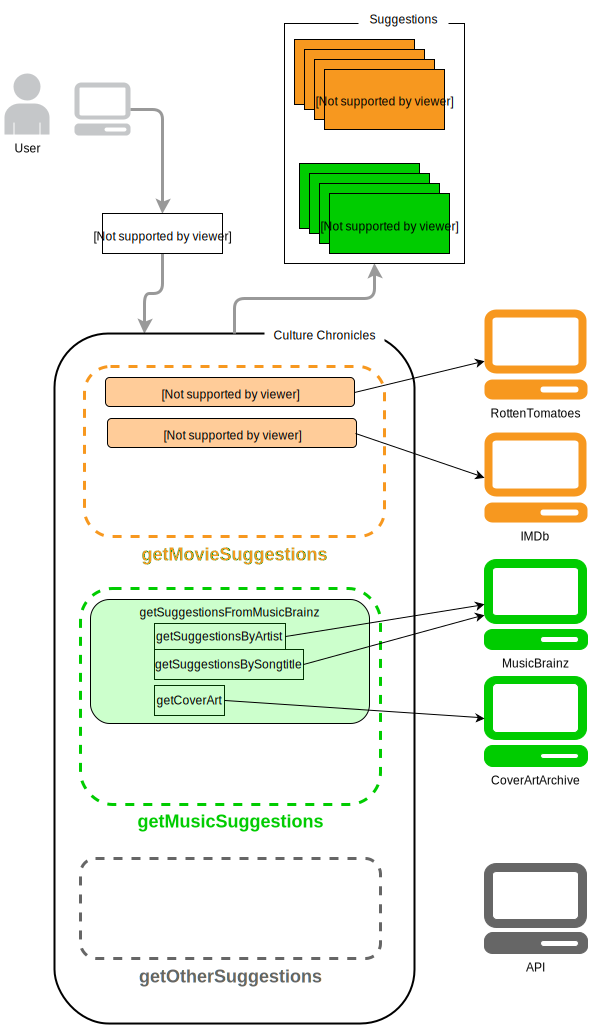
\includegraphics[width=0.7\textwidth]{RetrievingSuggestions.pdf}
		\caption{Suggestions - Request-Diagramm}
	\end{center}
	\label{fig:suggestionsRequestDiagram}
\end{figure}


\subsubsection{Erfassen von Suchergebnissen anhand eines Zeitraumes}
\label{subsec:results}
In Abbildung \ref{fig:searchResultsRequestDiagram} ist der interne Ablauf der Erfassung von Suchergebnissen schematisch dargestellt. Ausgangspunkt der Grafik ist ein bereits ausgew�hlter Zeitraum (\texttt{SuggestionDate}). Anhand des Datums wird mittels Scrapen der passenden \textbf{IMDb}-Seite eine Liste von IMDb-IDs erfasst. Alle restlichen Daten k�nnen mit Angabe der IMDb-ID von den APIs \textbf{RottenTomatoes} und \textbf{TrailerAddict} nachgeladen werden. Die Ergebnisse resultieren im Falle der Abfrage bei \textbf{RottenTomatoes} in einem Set von Movie-Results, im Falle der Abfrage von \textbf{TrailerAddict} in einer Liste von Trailern.\footnote{Genauer besteht die Liste von Trailern aus einer Liste von Quellcode-Snippets, die die eingebetteten Trailer-Videos enthalten.}

\begin{figure}[htb]
	\begin{center}
		\includegraphics[width=1\textwidth]{RetrievingSearchresultsAndPlaylist.pdf}
		\caption{Searchresults - Request-Diagramm}
	\end{center}
	\label{fig:searchResultsRequestDiagram}
\end{figure}


\subsubsection{Interne Daten�bertragung mittels MongoDB}
Da die in \arbeitstitel \ angezeigten und verarbeiteten Daten dynamisch von unterschiedlichen Quellen geladen werden sollen, ist eine Datenhaltung im Prinzip nicht erforderlich. Jedoch werden die zur Laufzeit erfassten Daten zwischengespeichert und intern auf Objekte gemappt.

Zu diesem Zweck wird die dokumentenorientierte Datenbank \textbf{MongoDB} \citep{mongodb} verwendet. Im Gegensatz zu relationalen Datenbanken l�sst sich mit der NoSQL-Strategie eine flexible Datenstruktur erstellen. Das macht im Falle von \arbeitstitel \ besonders Sinn, da sich Art und Umfang der Daten, die verarbeitet werden, sehr schnell �ndern k�nnen. Au�erdem vereinfacht dies auch die Erweiterbarkeit der Web-Applikation.

\paragraph{mongoose}
\textbf{mongoose} ist ein Objekt-Modellierungs-Tool f�r die Verwendung von MongoDB \citep{mongodb} unter Node.js. \citep[Vgl.][]{mongoose} Unter anderem bietet \textbf{mongoose} eine unkomplizierte, Schema-basierte L�sung zur Modellierung von Anwendungsdaten und verf�gt �ber Business-Logik, Funktionen wie das Typisieren, Validieren und vereinfacht das Formulieren von Datenbank-Queries \uvm \citep[Vgl.][]{mongoose}

\medskip
\begin{lstlisting}[language=JavaScript,caption=Deklaration des ResultItem mit Mongoose,label={lst:mongoose}]
var resultItemSchema = new Schema({
	mediaType: {type: String, enum: ['audio', 'video', 'text', 'other']},
	mediaSubtype: {type: String, enum: ['movie', 'music', 'time', 'other']},
	date: Date,
	title: String,
	img_url: String,
	id: String,
	source: String,
	url: String,
	release_mbid: String
});
\end{lstlisting}


\paragraph{SuggestionItem}
Bei Eingabe eines Suchbegriffes werden zun�chst die aktivierten APIs durchsucht. Dabei werden gleichzeitig multiple Suchanfragen an externe Datenquellen geschickt, wobei f�r jede API oder Datenquelle unterschiedliche Besonderheiten zu beachten sind. Um zu gew�hrleisten, dass eine Suchanfrage sowohl �ber die Eingabe eines Titels, als auch �ber die Eingabe des Interprets zum passenden Ergebnis f�hrt, werden zwei Suchanfragen gleichzeitig an die \textbf{MusicBrainz}-API geschickt. Dies liegt daran, dass die \textbf{MusicBrainz}-API die Angabe der Entit�t vorraussetzt, nach der gesucht werden soll. Das hei�t, dass eine Eingabe von \bspw \glqq Prince\grqq \ sowohl zu Songs des Interpreten \glqq Prince\grqq , als auch zu Songs, in denen das Wort \glqq Prince \grqq \ vorkommt.
\ref{fig:suggestionItem}

\begin{figure}[htb]
	\begin{center}
		\includegraphics[width=1\textwidth]{Klassendiagramm.pdf}
		\caption{Objekt-Diagramm des Suggestion-Objektes}
	\end{center}
	\label{fig:suggestionItem}
\end{figure}


\subsubsection{Erfassen von Medien-Items von externen Quellen}
Das Erfassen von Daten wird durch das Zusammenspiel mehrerer Module bewerkstelligt. Dies sind �ber die API-Wrapper hinaus die Module \textbf{async}, \textbf{node-rest-client}, \textbf{cheerio} und \textbf{request}.
Im Folgenden werden der Funktionsumfang und die Restriktionen der verwendeten API-Wrapper erl�utert. Daraufhin wird erkl�rt, inwiefern die zus�tzlichen Module zur Komplettierung der Implementierung n�tig sind.

\paragraph{NodeBrainz}
Das Node-Modul \textbf{NodeBrainz} ist ein schlanker Wrapper, der vollen Zugang zur MusicBrainz API (Version 2) bietet. \citep[Vgl.][]{nodebrainz} Dadurch wird eine komfortable Verwendung der \texttt{search}-Entit�t erm�glicht. Die Suche von Interpreten und Songtiteln wird mithilfe des \textbf{NodeBrainz}-Moduls bewerkstelligt.

\paragraph{Cover Art for Node}
Die CoverArt-API ist eine separate API von \textbf{MusicBrainz}, die das Nachschlagen von CoverArt anhand einer MusicBrainz-\texttt{release}-ID erm�glicht. Das Node-Modul \textbf{Cover Art for Node} implementiert diese Funktionalit�t und bietet zum einem die M�glichkeit Cover-Art in bin�rer Form zur�ck zu liefern, zum anderen ist es m�glich die gelieferten Bild-URLs zu Cover-Art in unterschiedlichen Gr��en zu erfassen. \citep{coverart}


\paragraph{node-imdb-api}
Da \textbf{IMDb} �ber keine offizelle API verf�gt, nutzt \citeauthor{nodeImdbApi} mehrere inoffizelle APIs, die Teile ihrer Daten aus den n�chtlich erscheinenden Daten der \textbf{IMDb} aggregieren. Da keine dieser APIs vollst�ndig ist, vereint \textbf{node-imdb-api} mehrere dieser RESTful APIs der inoffizellen Seiten. \citep[Vgl.][]{nodeImdbApi}

\paragraph{node-rest-client}
F�r Requests an die Schnittstelle \textbf{TrailerAddict} wird das Node-Modul \textbf{node-rest-client} verwendet. \citep{nodeRestClient} Es vereinfacht Requests an REST-APIs und liefert JavaScript-Objekte zur�ck, dessen Verarbeitung dann selbst �bernommen werden muss. Es erfordert zwar mehr Aufwand, einen Request durchzuf�hren, als einen API-Wrapper zu verwenden, da die Results eines Requests jedoch auch im Falle der Verwendung eines API-Wrappers erst auf die intern verwendeten Objekte gemappt werden m�ssen, ist der Mehraufwand vertretbar. Im Listing \ref{lst:nodeRestClient} ist der Aufruf der TrailerAddict-API anhand einer IMDb-ID zu sehen.

\medskip
\lstinputlisting[language=JavaScript,caption={Node-Rest-Client Beispiel},label={lst:nodeRestClient}]{Inhalt/Code/nodeRestClient.js}

\paragraph{Request}
Das Modul \textbf{Request} bewerkstelligt HTTP-Anfragen \citep{request} und dient in der Web-Applikation dem Erfassen des Quelltextes von \textbf{IMDb}, um die popul�rsten Filme eines spezifischen Jahres zu erfragen. Im Listing \ref{lst:request} ist zu sehen, wie der Quelltext der gegebenen IMDb-URL geladen wird.

\medskip
\lstinputlisting[language=JavaScript,caption={Request Beispiel},label={lst:request}]{Inhalt/Code/request.js}

\paragraph{cheerio}
Mithilfe des Node-Moduls \textbf{Cheerio} \citep{cheerio} lassen sich Informationen von Websites mittels CSS-Selektoren, wie sie in der Syntax von jQuery bekannt sind, erfassen. Die Verwendung dieser Bibliothek erleichtert das Web-Scraping \ua von \textbf{IMDb}. Im Listing \ref{lst:cheerio} ist zu sehen, wie die IMDb-IDs aus dem, durch das Scrapen erhaltenen Quelltext, erfasst werden. 

\medskip
\lstinputlisting[language=JavaScript,caption={Cheerio Beispiel},label={lst:cheerio}]{Inhalt/Code/cheerio.js}

\paragraph{async}
Das \textbf{async}-Modul \citep{async} erlaubt eine bessere Kontrolle �ber asynchron ausgef�hrte Funktionalit�t. Da \arbeitstitel \ an vielen Stellen mit mehreren APIs kommunizieren muss, ist die Asynchronit�t zwar generell ein Vorteil, jedoch werden auch Anfragen ben�tigt, die von mehreren asynchronen Requests abh�ngig sind. D.h., dass einige Requests von teilweise mehreren, vorangegangenen Requests abh�ngig sind. Mit async lassen sich Callbacks\footnote{Ein Callback ist eine ausf�hrbare \glqq Funktion, die einer anderen Funktion als Parameter �bergeben und von dieser unter gewissen Bedingungen wird.\grqq \citep[Vgl.][]{wikiCallback}} in vordefinierter Reihenfolge durchf�hren. Auch das Ausf�hren einer Serie von ein und dem selben Callback, um Werte einer Liste zu bearbeiten, ist m�glich. Genauso lassen sich mehrere Requests gleichzeitig abarbeiten, bis dann der finale Callback ausgef�hrt werden kann, wenn alle Vorbedingungen erf�llt worden sind.

Im Listing \ref{lst:async} ist zu sehen, wie das \texttt{async}-Modul zur parallelen Ausf�hrung von Funktionen beitr�gt. Die Funktionen \texttt{get""Music""Suggestions""By""Searchterm} und \texttt{get""Movie""Suggestions""By""Searchterm} werden parallel ausgef�hrt. Sobald beide Funktionen abgeschlossen sind und die jeweiligen Callback-Funktionen ausgef�hrt werden, wird das in Zeile \ref{lst:asyncCallback} implementierte Callback ausgef�hrt. �ber \texttt{results} kann auf die Ergebnisse der parallel ausgef�hrten Funktionen zugegriffen werden.

\medskip
\lstinputlisting[language=JavaScript,float,caption={Async Beispiel},label={lst:async}]{Inhalt/Code/async.js}

Au�erdem wird die von \textbf{async} bereitgestellte Funktion \texttt{each} verwendet. Auf diesem Wege kann f�r jedes Item eines Result-Sets, das von einer API bezogen wurde, ein Request ausgef�hrt werden, um \zB Cover-Art nachzuladen. Diese Funktion wird zum Abfragen der Film-Trailer verwendet, indem anhand eines Sets von \textbf{IMDb}-IDs f�r jeden gefundenen Film ein Trailer gesucht wird. Dies ist \ua im Listing \ref{lst:interaction} in Zeile \ref{lst:asyncEach} zu sehen.


\medskip
\lstinputlisting[language=JavaScript,float,caption={Request, Cheerio und Async in Action},label={lst:interaction}]{Inhalt/Code/requestCheerioAsync.js}


% ====

% HERE

% ====

\subsection{Einbinden weiterer Medientypen und Dienste}
Die Architektur des Servers ist zur einfachen Einbindung zus�tzlicher Medientypen und Datenquellen vorgesehen. Daf�r ist zum einen zwischen dem Einbinden eines neuen Medientyps und einer neuen Datenquelle zu unterscheiden. Desweiteren ist es m�glich eine Datenquelle lediglich f�r das Liefern von Suchvorschl�gen, zum Liefern von Suchergebnissen oder beidem einzubinden. Daf�r sind intern die Datenbank-Objekte \texttt{Suggestion} und \texttt{ResultItem} essentiell.

\paragraph{Einbinden eines Dienstes f�r Suchvorschl�ge}
F�r das Einbinden einer weiteren Schnittstelle zum Liefern von Suchvorschl�gen muss eine Funktion implementiert werden, die anhand des Parameters \texttt{String:searchTerm} eine Liste von \texttt{Suggestion}-Objekten (\texttt{List<Suggestion>:suggestions} zur�ck gibt. Werden die Ergebnisse der Suchvorschl�ge inklusive eines Icons oder Platzhalters f�r den implementierten Dienst und den Suchvorschlagdienst und die Quelle richtig angegeben, k�nnen die zus�tzlichen Suchvorschl�ge ohne Darstellungsfehler in der Selectbox angezeigt werden. Mithilfe von \textbf{mongoose} kann das resultierende Ergebnis eines neuen Dienstes auf ein \texttt{Suggestion}-Objekt gemappt werden (siehe Listing \ref{lst:imdbToSuggestion}).

\medskip
\lstinputlisting[float,language=JavaScript,caption={Mappen eines IMDb-Results zu einem Suggestion-Objekt},label={lst:imdbToSuggestion}]{Inhalt/Code/imdbToSuggestion.js}

\paragraph{Einbinden eines Dienstes f�r Suchergebnisse}
Das Einbinden einer weiteren Schnittstelle f�r Suchergebnisse ist �quivalent zur Einbindung eine weiteren Dienstes f�r Suchvorschl�ge. In diesem Fall wird als Parameter der Zeitpunkt mitgegeben\footnote{Derzeit ist dies die jeweilige Jahreszahl mit vier Stellen, \zB \glqq 1985\grqq \ oder \glqq 2014\grqq .} und eine Liste an \texttt{ResultItem}-Objekten (\texttt{List<ResultItem>:resultItems}) zur�ck geliefert.

Die implementierte Funktion wird dann im \texttt{async}-Rumpf eingebunden werden. Dies ist am Beispiel der Film-Suchvorschl�ge mit den beiden Diensten \textbf{IMDb} und \textbf{Rotten Tomatoes} in Listing \ref{lst:movieSuggestions} zu sehen.

\medskip
\lstinputlisting[float,language=JavaScript,caption={Einbinden von zus�tzlichen Diensten am Beispiel des Medientyps Film},label={lst:movieSuggestions}]{Inhalt/Code/getMovieSuggestionsBySearchterm.js}


\paragraph{Einbinden eines zus�tzlichen Medientyps}
Der Ablauf der Anfragen externer Dienste ist hierarchisch aufgebaut. So sind jeweils die Anfragen f�r Musik-Inhalte und Video-Inhalte in parallel ablaufenden Funktionen gruppiert, d.h. dass die einzelnen Dienste nach Medientyp sortiert abgefragt werden (siehe Listing \ref{lst:getSuggestions}).\footnote{Der genaue Ablauf f�r das Liefern von Suchvorschl�gen wird in der Grafik \ref{fig:suggestionsRequestDiagram} verdeutlicht, der Ablauf f�r das Liefern von Suchergebnissen wird in der Grafik \ref{fig:searchResultsRequestDiagram} dargestellt.} Das bedeutet, dass ein neuer Medientyp �quivalent eingebunden werden kann. Es muss eine Funktion implementiert werden, die die Abfragen der einzelnen Dienste, die den gleichen Medientyp liefern, b�ndelt. Das Ergebnis besteht aus einer Liste von \texttt{Suggestion}-Objekten. Diese Herangehensweise ist so gew�hlt worden, um das Feature der Eingrenzung nach Medientyp zu vereinfachen.

\medskip
\lstinputlisting[float,language=JavaScript,caption={Aufteilung der Requests an die externen Dienste nach Medientyp},label={lst:getSuggestions}]{Inhalt/Code/getSuggestions.js} 		%  20-30 Seiten
%     erforderliche/ben�tigte Quellen
%	m�gliche APIs und andere Quellen
%	m�gliche Frameworks f�r die Web-Applikation
%	Grobkonzept
%	Feinkonzept
%	Arbeitsweise
%!TEX root = ../Masterarbeit.tex
\chapter{Ergebnis}
\label{cha:ergebnis}
\begin{itemize}
	\item screenshots vom Prototypen
	\item was ist gut gelaufen, was ist schlecht gelaufen, wo wurde gespart
\end{itemize}				% 3-10 Seiten
%!TEX root = ../Masterarbeit.tex
\chapter{Ausblick}
\label{cha:ausblick}


\section{Problematik und Weiterentwicklung} % Ausblick
\section{Fazit und kritische Bewertung} % Fazit		% 3-5 Seiten
% Ausblick
% Fazit





%%!TEX root = ../Masterarbeit.tex
\chapter{Zitate und Referenzen}
\label{cha:ZitateReferenzen}

Die \NeuerBegriff{Service-orientierte Architektur} (SOA) ist seit einiger Zeit \textit{das} Schlagwort im Bereich der Informationstechnologie. So haben \zB Deutschlands gr��te Softwarehersteller SAP und die Software AG ihre Unternehmensstrategie komplett auf die SOA ausgerichtet. \Autor{SAP2007} bietet mit \Fachbegriff{Netweaver} seine marktf�hrende ERP-Software auf Basis von SOA an,\footnote{\Vgl\Zitat[S.~127]{SAP2007}} und die \Autor{Software2007b}, die sich selbst als "`The XML Company"' bezeichnet, erweiterte k�rzlich noch einmal ihr bereits durchg�ngig an der SOA orientiertes Produktportfolio durch den Kauf des amerikanischen Unternehmens webMethods um L�sungen zur Unterst�tzung von Gesch�ftsprozessen.\footnote{\Vgl\Zitat{Software2007b}} In einem Atemzug mit der SOA werden h�ufig Webservices genannt, da sie durch ihre hohe Plattformunabh�ngigkeit und den Einsatz von Internettechnologie oftmals als Referenzimplementierung f�r die Services in einer SOA angef�hrt werden. Doch welche Vorteile bietet der Einsatz von Webservices in Unternehmen? K�nnen mit ihnen tats�chlich flexiblere Softwaresysteme entwickelt werden? Und wie einfach ist die Implementierung von Webservices auf unterschiedlichen Plattformen? Diesen Fragen wird sich der Autor in der vorliegenden Arbeit widmen.

\begin{wrapfigure}{l}{0.5\textwidth}
  \begin{center}
    \includegraphics[width=0.48\textwidth]{screens/09_home.jpg}
  \end{center}
  \caption{Home-Screen von dem der Spieler in alle Menu-Punkte navigieren kann.}
\end{wrapfigure}

Wie bereits in Kapitel \ref{cha:Einleitung} auf Seite \pageref{cha:Einleitung} erw�hnt, ist zur Unterst�tzung von Gesch�ftsprozessen der Einsatz von Informationstechnologie notwendig. Der Autor verfolgt mit dieser Arbeit das Ziel, einen Gesch�ftsprozess \todo{Was ist ein Gesch�ftsprozess?} mit Hilfe von Webservices zu optimieren. Hierzu wird er in diesem Kapitel eine Einf�hrung in das Thema Webservices und die damit in Zusammenhang stehenden Technologien geben, und auch auf m�gliche Einsatzbereiche von Webservices im Rahmen der Gesch�ftsprozessoptimierung eingehen. Tabelle \ref{tab:ElementeDerEreignisgesteuertenProzesskette} auf Seite \pageref{tab:ElementeDerEreignisgesteuertenProzesskette} zeigt ganz tolle Sachen.

Ich empfehle allen Softwareentwicklern die Lekt�re von \Zitat{Goodliffe2007}.

\section{Definitionen}
Die Service-orientierte Architektur ist ein Ansatz der Softwareentwicklung, der sich stark am Konzept der Gesch�ftsprozesse orientiert und mit Hilfe von Webservices implementiert werden kann. In den beiden folgenden Kapiteln werden beide Begriffe eingehend erl�utert, worauf in Kapitel \ref{cha:Fazit} die f�r die Umsetzung von Webservices ben�tigten Technologien vorgestellt werden.

\section{Service-orientierte Architektur}
\Autor{OASIS2007}\footnote{Die \NeuerBegriff{Organization for the Advancement of Structured Information Standards} ist nach \Zitat{OASIS2007} ein internationales Konsortium aus �ber 600 Organisationen, das sich der Entwicklung von E-Business-Standards verschrieben hat. Mitglieder sind \zB IBM, SAP und Sun.} definiert den Begriff \NeuerBegriff{Service-orientierte Architektur} (SOA) wie folgt:
\begin{quote}
"`\textbf{Service Oriented Architecture} [\ldots] is a paradigm for organizing and utilizing distributed \textbf{capabilities} that may be under the control of different ownership domains."'\footnote{\Zitat[S.~8]{OASIS2006a}}
\end{quote}
Diese bewusst allgemein gehaltene Definition stammt aus dem Referenzmodell der SOA aus dem Jahr 2006. Dieses Modell wurde mit dem Ziel entwickelt, ein einheitliches Verst�ndnis des Begriffs SOA und des verwendeten Vokabulars zu schaffen, und sollte die zahlreichen bis dato vorhandenen, teils widerspr�chlichen Definitionen abl�sen.\footnote{\Vgl\Zitat[S.~4]{OASIS2006a}} Dabei wird zun�chst noch kein Bezug zur Informationstechnologie hergestellt, sondern allgemein von F�higkeiten gesprochen, die Personen, Unternehmen, aber eben auch Computer besitzen und evtl. Anderen anbieten, um Probleme zu l�sen. Als Beispiel wird ein Energieversorger angef�hrt, der Haushalten seine F�higkeit Strom zu erzeugen anbietet.\footnote{\Vgl\Zitat[S.~8f.]{OASIS2006a}}



\chapter{Bilder und Listings}

In den folgenden drei Kapiteln wird der Autor eine einfache Webservice-Umgebung aufbauen, um zu zeigen, wie Webservices in der Praxis angeboten, konsumiert und orchestriert werden k�nnen. Hierzu verwendet er ausschlie�lich Open-Source-Software, im Speziellen \NeuerBegriff{Apache Tomcat}\footnote{Website: \url{http://tomcat.apache.org/}} als Servlet-Engine, \NeuerBegriff{Apache Axis2}\footnote{Website: \url{http://ws.apache.org/axis2/}} als SOAP-Engine und \NeuerBegriff{ActiveBPEL}\footnote{Website: \url{http://www.activebpel.org/}} als Workflow-System. Die Installation und Konfiguration der ben�tigten Anwendungen wird in Kapitel \ref{sec:Werkzeuge} beschrieben. Die komplette Umgebung inkl. der vom Autor erstellten Webservices befindet sich als virtuelle Maschine auf der dieser Arbeit beigelegten DVD. Im Folgenden wird der DNS-Name \Code{linux-ws} als Bezeichnung f�r den Webservice-Server verwendet.

\section{Anbieten eines Webservice}
\label{sec:AnbietenEinesWebservices}
Mit Hilfe von Apache Axis2 k�nnen Webservices sehr einfach auf Basis von normalen Java-Klassen angeboten werden. Es ist lediglich eine zus�tzliche XML-Datei namens \Datei{META-INF/services.xml} n�tig, in der die zu ver�ffentlichenden Klassen und Methoden beschrieben werden. \abbildung{HelloWorldStruktur} zeigt die Struktur eines einfachen \Webservice{HelloWorld}-Webservice.

\begin{figure}[htb]
\centering
\includegraphics[width=0.3\textwidth]{HelloWorldStruktur.jpg}
\caption{\Webservice{HelloWorld}-Webservice: Dateistruktur}
\label{fig:HelloWorldStruktur}
\end{figure}

Die Klasse \Code{HelloWorld} besitzt nur die Methode \Code{SayHello}, die den \Datentyp{String} \Code{Hello World!} zur�ckgibt. Sie wird in Listing \ref{lst:HelloWorldJava} gezeigt. 

\newpage
\lstset{language=Java, basicstyle=\footnotesize, showstringspaces=false, tabsize=2}
\lstinputlisting[label=lst:HelloWorldJava,caption=\Webservice{HelloWorld}-Webservice: Java-Klasse \Code{HelloWorld}]{DVD/Listings/HelloWorld/HelloWorld.java}

\section{Netzwerkverkehr beim Aufruf von \Webservice{PersonFactory}}

\subsection{SOAP-Request}
Listing \ref{lst:SOAPRequest} zeigt die mitgeschnittene SOAP-Anfrage per HTTP an den Webservice \Webservice{PersonFactory}. Wie am Ende von Kapitel \ref{cha:Einleitung} beschrieben, wird die eigentliche SOAP-Nachricht mittels des HTTP-\Eingabe{POST}-Befehls (Zeile 1) an den Webservice unter der angegebenen URL (Zeile 1) auf dem Server (Zeile 5) geschickt. In Zeile 3 wird �ber den Befehl \Eingabe{SOAPAction} �bermittelt, welche Funktion des Webservice (in diesem Fall \Code{CreatePerson}) aufgerufen werden soll. Die XML-Nutzlast (Zeilen 8--18) besteht dann aus einer einfachen SOAP-Nachricht aus \XMLElement{Envelope}, \XMLElement{Header} und \XMLElement{Body}, die einen RPC durchf�hrt. Die aufzurufenden Funktion wird noch einmal im SOAP-\XMLElement{Body} in Zeile 15 definiert.


\lstset{language=XML, basicstyle=\footnotesize, showstringspaces=false, tabsize=2}
\lstinputlisting[label=lst:SOAPRequest,caption=SOAP-Request an \Webservice{PersonFactory} per HTTP]{DVD/Listings/PersonFactorySOAPRequest.txt}

\subsection{SOAP-Response}
Die Antwort des \Webservice{PersonFactory}-Webservice zeigt Listing \ref{lst:SOAPResponse}. Sie beginnt in Zeile 1 mit dem HTTP-Statuscode 200, der die Anfrage als erfolgreich kennzeichnet. Die eigentliche Nutzlast in Form von XML-Daten (Zeile 3) folgt dann ab Zeile 7. Sie besteht aus dem Element \XMLElement{Person} und seinen Unterelementen, umschlossen vom Element \XMLElement{CreatePersonRepsonse}, das die Antwort-Nachricht aus der WSDL repr�sentiert.

\lstset{language=XML, basicstyle=\footnotesize, showstringspaces=false, tabsize=2}
\lstinputlisting[label=lst:SOAPResponse,caption=SOAP-Response von \Webservice{PersonFactory} per HTTP]{DVD/Listings/PersonFactorySOAPResponse.txt}





\chapter{Aufz�hlungen und Tabellen}


Eine normale Punktliste:
\begin{itemize}
\item Lorem ipsum dolor sit amet, consectetuer adipiscing elit. Nulla ac ipsum a metus viverra tempor. 
\item Nunc sem. Nulla nec urna eu nibh vehicula convallis. Integer ac turpis. Donec mauris enim, dignissim quis, scelerisque ac, rhoncus id, sapien. 
\item Donec turpis felis, cursus in, varius vitae, mollis ac, lorem. Integer a dui sit amet eros nonummy aliquet. Donec egestas adipiscing tellus. Nulla iaculis. 
\item Aliquam erat volutpat. Curabitur posuere, eros vitae accumsan semper, risus erat viverra erat, eu vehicula mi leo at elit. Fusce luctus. Fusce vehicula pretium diam. Nunc sed arcu ut erat suscipit fermentum.
\end{itemize}

Eine nummerierte Liste:
\begin{enumerate}
\item Lorem ipsum dolor sit amet, consectetuer adipiscing elit. Nulla ac ipsum a metus viverra tempor. 
\item Nunc sem. Nulla nec urna eu nibh vehicula convallis. Integer ac turpis. Donec mauris enim, dignissim quis, scelerisque ac, rhoncus id, sapien. 
\item Donec turpis felis, cursus in, varius vitae, mollis ac, lorem. Integer a dui sit amet eros nonummy aliquet. Donec egestas adipiscing tellus. Nulla iaculis. 
\item Aliquam erat volutpat. Curabitur posuere, eros vitae accumsan semper, risus erat viverra erat, eu vehicula mi leo at elit. Fusce luctus. Fusce vehicula pretium diam. Nunc sed arcu ut erat suscipit fermentum.
\end{enumerate}

\begin{enumerate}[a)]
\item Diese Liste...
\item ...hat anstatt der normalen schwarzen Punkte...
\item ...Buchstaben als Marker.
\end{enumerate}


\section{Vom Autor verwendete Software}
\label{sec:Werkzeuge}
Im Folgenden werden die Programme vorgestellt, die der Autor zum Erstellen dieser Arbeit und vor allem zur Entwicklung der Webservices verwendet hat. Soweit es m�glich war, wurden Open-Source-Programme eingesetzt.

\begin{itemize}
\itemd{Microsoft Visio}{Die EPKs der BAP wurden mit Microsoft Visio erstellt. Der Autor hat zwar verschiedene Open-Source-Programme\footnote{Dia, OpenOffice Draw und die EPC Tools.} ausprobiert, mit denen EPKs erstellt werden k�nnten, die grafischen Ergebnisse waren aber nicht zufriedenstellend. Die Symbole von Visio sehen den "`originalen"' ARIS-Symbolen am �hnlichsten und k�nnen dar�ber hinaus mit zus�tzlichen Informationen wie Dauer und Kosten versehen werden.}
\itemd{PSPad}{F�r die Bearbeitung von verschiedenen (Text-)Dateien wurde der Texteditor PSPad verwendet. Mit diesem konnten \zB auch die regul�ren Ausdr�cke f�r die XML-Schemas entwickelt werden. Website: \url{http://www.pspad.com/}}
\itemd{Eclipse}{Sowohl der ActiveBPEL Designer als auch die EntireX Workbench sind Plugins f�r die IDE Eclipse. Auch zur Java- und PHP-Entwicklung wurde dieses Werkzeug verwendet. Website: \url{http://www.eclipse.org/}}
\itemd{XML Copy Editor}{F�r die Entwicklung der XML-Schemas und die Bearbeitung von XML-Dateien wurde der XML Copy Editor eingesetzt. Mit diesem k�nnen \ua XML-Dateien auf Wohlgeformtheit gepr�ft und gegen ihr Schema validiert werden. Website: \url{http://xml-copy-editor.sourceforge.net/}}
\itemd{soapUI}{
Mit soapUI k�nnen Webservices getestet werden, ohne einen Client zu programmieren. Die SOAP-Anfragen werden automatisch anhand der WSDL generiert und die Antworten k�nnen gegen die WSDL-Datei validiert werden. Website: \url{http://www.soapui.org/}}
\itemd{Ethereal}{
Die Netzwerkkommunikation beim Aufrufen der Webservices wurde mit Ethereal, einem umfangreichen Werkzeug zur Analyse des Netzwerkverkehrs, mitgeschnitten. Website: \url{http://www.ethereal.com/}}
\itemd{\LaTeX}{
Diese Arbeit wurde mit {\LaTeX} geschrieben. Als Distribution wurde MiKTeX verwendet und als Editor der LaTeX Editor. Websites: \url{http://miktex.org/}, \url{http://www.latexeditor.org/}}
\end{itemize}

\section{Elemente der Ereignisgesteuerten Prozesskette}

\begin{longtable}{|m{10cm}|m{3cm}|}
\caption{Elemente der Ereignisgesteuerten Prozesskette} \\
\hline
\label{tab:ElementeDerEreignisgesteuertenProzesskette}
\textbf{Element} & \textbf{Symbol}\\
\hline
\textbf{Funktion} 

Funktionen beschreiben T�tigkeiten, die im Verlauf des Gesch�ftsprozesses anfallen. Sie k�nnen von Mitarbeitern oder einem Informationssystem durchgef�hrt werden und ben�tigen evtl. Ressourcen, die ihnen zugewiesen werden. 

Beispiele: \textit{Auftrag anlegen}, \textit{Rechnung schreiben}, \textit{Konto abschlie�en} & 
\includegraphics[width=3cm]{EPK-Funktion.jpg} \\
\hline
\textbf{Ereignis} 

Ereignisse sind betriebswirtschaftlich relevante Ereignisse, die den Gesch�ftsprozess in irgendeiner Weise steuern oder beeinflussen. Ereignisse sind immer Ausl�ser oder Ergebnisse von Funktionen. Ein Gesch�ftsprozess beginnt und endet stets mit einem Ereignis. 

Beispiele: \textit{Auftrag eingetroffen}, \textit{�berweisung get�tigt}, \textit{Rechnung erstellt} & 
\includegraphics[width=3cm]{EPK-Ereignis.jpg} \\
\hline
\textbf{Operatoren} 

Operatoren steuern den Kontrollfluss eines Gesch�ftsprozesses. Sie machen \zB deutlich, dass eine Funktion mehrere Ereignisse ausl�st, oder zeigen alternative Vorgehensweisen an. Es gibt drei Operatoren (v.\,l.\,n.\,r.\,): UND, ODER und XODER (exklusives ODER). & 
\includegraphics[width=3cm]{EPK-Operatoren.jpg} \\
\hline
\textbf{Organisationseinheit} 

Organisationseinheiten werden Funktionen zugeordnet und beschreiben, wo die Funktionen ausgef�hrt werden bzw. wer sie ausf�hrt. Die Bezeichnung der Symbole enth�lt zus�tzlich zur Abteilung noch die Namen der Mitarbeiter.

Beispiele: \textit{Vertrieb}, \textit{Personal}, \textit{Produktion} & 
\includegraphics[width=3cm]{EPK-Organisationseinheit.jpg} \\
\hline
\textbf{Informationsobjekt} 

Auch Informationsobjekte werden Funktionen zugewiesen und beschreiben die von diesen ben�tigten oder erstellten Informationen. Dabei sind s�mtliche Formen von Informationen auf verschiedenen Datentr�gern m�glich und nicht etwa nur digitale Daten. Die Bezeichnung der Symbole enth�lt zus�tzlich das Informationssystem, aus dem die Informationen stammen.

Beispiele: \textit{Kundendatenbank}, \textit{Versicherungsantrag}, \textit{Rechnung} & 
\includegraphics[width=3cm]{EPK-Informationen.jpg} \\
\hline
\textbf{Prozesswegweiser}

Mit Prozesswegweisern werden Prozesse, die in anderen EPKs beschrieben sind, referenziert. So k�nnen \zB un�bersichtliche Prozesse in Teilprozesse gegliedert und h�ufig verwendete Prozesse an zentraler Stelle modelliert werden. Prozesswegweiser stehen in einer EPK immer anstelle von Funktionen. & 
\includegraphics[width=3cm]{EPK-Prozesspfad.jpg} \\
\hline
\end{longtable}